% ----------------------------------------------------------------------
%
%                            TFMTesis.tex
%
%----------------------------------------------------------------------
%
% Este fichero contiene el "documento maestro" del documento. Lo único
% que hace es configurar el entorno LaTeX e incluir los ficheros .tex
% que contienen cada sección.
%
%----------------------------------------------------------------------
% rm -rf *.idx *.lof *.log *.out *.synctex.gz *.toc *.bst *.aux *.bbl
% Los ficheros necesarios para este documento son:
%
%       TeXiS/* : ficheros de la plantilla TeXiS.
%       Cascaras/* : ficheros con las partes del documento que no
%          son capítulos ni apéndices (portada, agradecimientos, etc.)
%       Capitulos/*.tex : capítulos de la tesis
%       Apendices/*.tex: apéndices de la tesis
%       constantes.tex: constantes LaTeX
%       config.tex : configuración de la "compilación" del documento
%       guionado.tex : palabras con guiones
%
% Para la bibliografía, además, se necesitan:
%
%       *.bib : ficheros con la información de las referencias
%
% ---------------------------------------------------------------------

\documentclass[12pt,a4paper,twoside]{book}

%
% Definimos  el   comando  \compilaCapitulo,  que   luego  se  utiliza
% (opcionalmente) en config.tex. Quedaría  mejor si también se definiera
% en  ese fichero,  pero por  el modo  en el  que funciona  eso  no es
% posible. Puedes consultar la documentación de ese fichero para tener
% más  información. Definimos también  \compilaApendice, que  tiene el
% mismo  cometido, pero  que se  utiliza para  compilar  únicamente un
% apéndice.
%
%
% Si  queremos   compilar  solo   una  parte  del   documento  podemos
% especificar mediante  \includeonly{...} qué ficheros  son los únicos
% que queremos  que se incluyan.  Esto  es útil por  ejemplo para sólo
% compilar un capítulo.
%
% El problema es que todos aquellos  ficheros que NO estén en la lista
% NO   se  incluirán...  y   eso  también   afecta  a   ficheros  de
% la plantilla...
%
% Total,  que definimos  una constante  con los  ficheros  que siempre
% vamos a querer compilar  (aquellos relacionados con configuración) y
% luego definimos \compilaCapitulo.
\newcommand{\ficherosBasicosTeXiS}{%
TeXiS/TeXiS_pream,TeXiS/TeXiS_cab,TeXiS/TeXiS_bib,TeXiS/TeXiS_cover%
}
\newcommand{\ficherosBasicosTexto}{%
constantes,guionado,Cascaras/bibliografia,config%
}
\newcommand{\compilaCapitulo}[1]{%
\includeonly{\ficherosBasicosTeXiS,\ficherosBasicosTexto,Capitulos/#1}%
}

\newcommand{\compilaApendice}[1]{%
\includeonly{\ficherosBasicosTeXiS,\ficherosBasicosTexto,Apendices/#1}%
}

%- - - - - - - - - - - - - - - - - - - - - - - - - - - - - - - - - - -
%            Preámbulo del documento. Configuraciones varias
%- - - - - - - - - - - - - - - - - - - - - - - - - - - - - - - - - - -

% Define  el  tipo  de  compilación que  estamos  haciendo.   Contiene
% definiciones  de  constantes que  cambian  el  comportamiento de  la
% compilación. Debe incluirse antes del paquete TeXiS/TeXiS.sty
%---------------------------------------------------------------------
%
%                          config.tex
%
%---------------------------------------------------------------------
%
% Contiene la  definición de constantes  que determinan el modo  en el
% que se compilará el documento.
%
%---------------------------------------------------------------------
%
% En concreto, podemos  indicar si queremos "modo release",  en el que
% no  aparecerán  los  comentarios  (creados  mediante  \com{Texto}  o
% \comp{Texto}) ni los "por  hacer" (creados mediante \todo{Texto}), y
% sí aparecerán los índices. El modo "debug" (o mejor dicho en modo no
% "release" muestra los índices  (construirlos lleva tiempo y son poco
% útiles  salvo  para   la  versión  final),  pero  sí   el  resto  de
% anotaciones.
%
% Si se compila con LaTeX (no  con pdflatex) en modo Debug, también se
% muestran en una esquina de cada página las entradas (en el índice de
% palabras) que referencian  a dicha página (consulta TeXiS_pream.tex,
% en la parte referente a show).
%
% El soporte para  el índice de palabras en  TeXiS es embrionario, por
% lo  que no  asumas que  esto funcionará  correctamente.  Consulta la
% documentación al respecto en TeXiS_pream.tex.
%
%
% También  aquí configuramos  si queremos  o  no que  se incluyan  los
% acrónimos  en el  documento final  en la  versión release.  Para eso
% define (o no) la constante \acronimosEnRelease.
%
% Utilizando \compilaCapitulo{nombre}  podemos también especificar qué
% capítulo(s) queremos que se compilen. Si no se pone nada, se compila
% el documento  completo.  Si se pone, por  ejemplo, 01Introduccion se
% compilará únicamente el fichero Capitulos/01Introduccion.tex
%
% Para compilar varios  capítulos, se separan sus nombres  con comas y
% no se ponen espacios de separación.
%
% En realidad  la macro \compilaCapitulo  está definida en  el fichero
% principal tesis.tex.
%
%---------------------------------------------------------------------


% Comentar la línea si no se compila en modo release.
% TeXiS hará el resto.
% ¡¡¡Si cambias esto, haz un make clean antes de recompilar!!!
%\def\release{1}


% Descomentar la linea si se quieren incluir los
% acrónimos en modo release (en modo debug
% no se incluirán nunca).
% ¡¡¡Si cambias esto, haz un make clean antes de recompilar!!!
%\def\acronimosEnRelease{1}


% Descomentar la línea para establecer el capítulo que queremos
% compilar

% \compilaCapitulo{introduccion}


% \compilaApendice{ApendiceA}

% Variable local para emacs, para  que encuentre el fichero maestro de
% compilación y funcionen mejor algunas teclas rápidas de AucTeX
%%%
%%% Local Variables:
%%% mode: latex
%%% TeX-master: "./Tesis.tex"
%%% End:


% Paquete de la plantilla
\usepackage{./TeXiS/TeXiS}

%PAQUETES PERSONALIZADOS
\usepackage{multicol}

% Incluimos el fichero con comandos de constantes
%---------------------------------------------------------------------
%
%                          constantes.tex
%
%---------------------------------------------------------------------
%
% Fichero que  declara nuevos comandos LaTeX  sencillos realizados por
% comodidad en la escritura de determinadas palabras
%
%---------------------------------------------------------------------

%%%%%%%%%%%%%%%%%%%%%%%%%%%%%%%%%%%%%%%%%%%%%%%%%%%%%%%%%%%%%%%%%%%%%%
% Comando: 
%
%       \titulo
%
% Resultado: 
%
% Escribe el título del documento.
%%%%%%%%%%%%%%%%%%%%%%%%%%%%%%%%%%%%%%%%%%%%%%%%%%%%%%%%%%%%%%%%%%%%%%
\def\titulo{Predicción de Riesgo Cardiovascular Explicable mediante \emph{Deep Learning}}

%%%%%%%%%%%%%%%%%%%%%%%%%%%%%%%%%%%%%%%%%%%%%%%%%%%%%%%%%%%%%%%%%%%%%%
% Comando: 
%
%       \autor
%
% Resultado: 
%
% Escribe el autor del documento.
%%%%%%%%%%%%%%%%%%%%%%%%%%%%%%%%%%%%%%%%%%%%%%%%%%%%%%%%%%%%%%%%%%%%%%
\def\autor{Noelia Barranco Godoy}

% Variable local para emacs, para  que encuentre el fichero maestro de
% compilación y funcionen mejor algunas teclas rápidas de AucTeX

%%%
%%% Local Variables:
%%% mode: latex
%%% TeX-master: "TFGTeXiS.tex"
%%% End:


% Sacamos en el log de la compilación el copyright
%\typeout{Copyright Marco Antonio and Pedro Pablo Gomez Martin}

%
% "Metadatos" para el PDF
%
\ifpdf\hypersetup{%
    pdftitle = {\titulo},
    pdfsubject = {Trabajo de Fin de Grado de Noelia Barranco Godoy},
    pdfkeywords = {Redes neuronales, ECG, TFG},
    pdfauthor = {\textcopyright\ \autor},
    pdfcreator = {\LaTeX\ con el paquete \flqq hyperref\frqq},
    pdfproducer = {pdfeTeX-0.\the\pdftexversion\pdftexrevision},
    }
    \pdfinfo{/CreationDate (\today)}
\fi


%- - - - - - - - - - - - - - - - - - - - - - - - - - - - - - - - - - -
%                        Documento
%- - - - - - - - - - - - - - - - - - - - - - - - - - - - - - - - - - -
\begin{document}

% Incluimos el  fichero de definición de guionado  de algunas palabras
% que LaTeX no ha dividido como debería
%----------------------------------------------------------------
%
%                          guionado.tex
%
%----------------------------------------------------------------
%
% Fichero con algunas divisiones de palabras que LaTeX no
% hace correctamente si no se le da alguna ayuda.
%
%----------------------------------------------------------------

\hyphenation{
% a
abs-trac-to
abs-trac-tos
abs-trac-ta
abs-trac-tas
ac-tua-do-res
a-gra-de-ci-mien-tos
ana-li-za-dor
an-te-rio-res
an-te-rior-men-te
apa-rien-cia
a-pro-pia-do
a-pro-pia-dos
a-pro-pia-da
a-pro-pia-das
a-pro-ve-cha-mien-to
a-que-llo
a-que-llos
a-que-lla
a-que-llas
a-sig-na-tu-ra
a-sig-na-tu-ras
a-so-cia-da
a-so-cia-das
a-so-cia-do
a-so-cia-dos
au-to-ma-ti-za-do
% b
batch
bi-blio-gra-fía
bi-blio-grá-fi-cas
bien
bo-rra-dor
boo-l-ean-expr
% c
ca-be-ce-ra
call-me-thod-ins-truc-tion
cas-te-lla-no
cir-cuns-tan-cia
cir-cuns-tan-cias
co-he-ren-te
co-he-ren-tes
co-he-ren-cia
co-li-bri
co-men-ta-rio
co-mer-cia-les
co-no-ci-mien-to
cons-cien-te
con-si-de-ra-ba
con-si-de-ra-mos
con-si-de-rar-se
cons-tan-te
cons-trucción
cons-tru-ye
cons-tru-ir-se
con-tro-le
co-rrec-ta-men-te
co-rres-pon-den
co-rres-pon-dien-te
co-rres-pon-dien-tes
co-ti-dia-na
co-ti-dia-no
crean
cris-ta-li-zan
cu-rri-cu-la
cu-rri-cu-lum
cu-rri-cu-lar
cu-rri-cu-la-res
% d
de-di-ca-do
de-di-ca-dos
de-di-ca-da
de-di-ca-das
de-rro-te-ro
de-rro-te-ros
de-sa-rro-llo
de-sa-rro-llos
de-sa-rro-lla-do
de-sa-rro-lla-dos
de-sa-rro-lla-da
de-sa-rro-lla-das
de-sa-rro-lla-dor
de-sa-rro-llar
des-cri-bi-re-mos
des-crip-ción
des-crip-cio-nes
des-cri-to
des-pués
de-ta-lla-do
de-ta-lla-dos
de-ta-lla-da
de-ta-lla-das
di-a-gra-ma
di-a-gra-mas
di-se-ños
dis-po-ner
dis-po-ni-bi-li-dad
do-cu-men-ta-da
do-cu-men-to
do-cu-men-tos
% e
edi-ta-do
e-du-ca-ti-vo
e-du-ca-ti-vos
e-du-ca-ti-va
e-du-ca-ti-vas
e-la-bo-ra-do
e-la-bo-ra-dos
e-la-bo-ra-da
e-la-bo-ra-das
es-co-llo
es-co-llos
es-tu-dia-do
es-tu-dia-dos
es-tu-dia-da
es-tu-dia-das
es-tu-dian-te
e-va-lua-cio-nes
e-va-lua-do-res
exis-ten-tes
exhaus-ti-va
ex-pe-rien-cia
ex-pe-rien-cias
% f
for-ma-li-za-do
% g
ge-ne-ra-ción
ge-ne-ra-dor
ge-ne-ra-do-res
ge-ne-ran
% h
he-rra-mien-ta
he-rra-mien-tas
% i
i-dio-ma
i-dio-mas
im-pres-cin-di-ble
im-pres-cin-di-bles
in-de-xa-do
in-de-xa-dos
in-de-xa-da
in-de-xa-das
in-di-vi-dual
in-fe-ren-cia
in-fe-ren-cias
in-for-ma-ti-ca
in-gre-dien-te
in-gre-dien-tes
in-me-dia-ta-men-te
ins-ta-la-do
ins-tan-cias
% j
% k
% l
len-gua-je
li-be-ra-to-rio
li-be-ra-to-rios
li-be-ra-to-ria
li-be-ra-to-rias
li-mi-ta-do
li-te-ra-rio
li-te-ra-rios
li-te-ra-ria
li-te-ra-rias
lo-tes
% m
ma-ne-ra
ma-nual
mas-que-ra-de
ma-yor
me-mo-ria
mi-nis-te-rio
mi-nis-te-rios
mo-de-lo
mo-de-los
mo-de-la-do
mo-du-la-ri-dad
mo-vi-mien-to
% n
na-tu-ral
ni-vel
nues-tro
% o
obs-tan-te
o-rien-ta-do
o-rien-ta-dos
o-rien-ta-da
o-rien-ta-das
% p
pa-ra-le-lo
pa-ra-le-la
par-ti-cu-lar
par-ti-cu-lar-men-te
pe-da-gó-gi-ca
pe-da-gó-gi-cas
pe-da-gó-gi-co
pe-da-gó-gi-cos
pe-rio-di-ci-dad
per-so-na-je
plan-te-a-mien-to
plan-te-a-mien-tos
po-si-ción
pre-fe-ren-cia
pre-fe-ren-cias
pres-cin-di-ble
pres-cin-di-bles
pri-me-ra
pro-ble-ma
pro-ble-mas
pró-xi-mo
pu-bli-ca-cio-nes
pu-bli-ca-do
% q
% r
rá-pi-da
rá-pi-do
ra-zo-na-mien-to
ra-zo-na-mien-tos
re-a-li-zan-do
re-fe-ren-cia
re-fe-ren-cias
re-fe-ren-cia-da
re-fe-ren-cian
re-le-van-tes
re-pre-sen-ta-do
re-pre-sen-ta-dos
re-pre-sen-ta-da
re-pre-sen-ta-das
re-pre-sen-tar-lo
re-qui-si-to
re-qui-si-tos
res-pon-der
res-pon-sa-ble
% s
se-pa-ra-do
si-guien-do
si-guien-te
si-guien-tes
si-guie-ron
si-mi-lar
si-mi-la-res
si-tua-ción
% t
tem-pe-ra-ments
te-ner
trans-fe-ren-cia
trans-fe-ren-cias
% u
u-sua-rio
Unreal-Ed
% v
va-lor
va-lo-res
va-rian-te
ver-da-de-ro
ver-da-de-ros
ver-da-de-ra
ver-da-de-ras
ver-da-de-ra-men-te
ve-ri-fi-ca
% w
% x
% y
% z
}
% Variable local para emacs, para que encuentre el fichero
% maestro de compilación
%%%
%%% Local Variables:
%%% mode: latex
%%% TeX-master: "./Tesis.tex"
%%% End:


% Marcamos  el inicio  del  documento para  la  numeración de  páginas
% (usando números romanos para esta primera fase).
\frontmatter
\pagestyle{empty}

%---------------------------------------------------------------------
%
%                          configCover.tex
%
%---------------------------------------------------------------------
%
% cover.tex
% Copyright 2009 Marco Antonio Gomez-Martin, Pedro Pablo Gomez-Martin
%
% This file belongs to the TeXiS manual, a LaTeX template for writting
% Thesis and other documents. The complete last TeXiS package can
% be obtained from http://gaia.fdi.ucm.es/projects/texis/
%
% Although the TeXiS template itself is distributed under the 
% conditions of the LaTeX Project Public License
% (http://www.latex-project.org/lppl.txt), the manual content
% uses the CC-BY-SA license that stays that you are free:
%
%    - to share & to copy, distribute and transmit the work
%    - to remix and to adapt the work
%
% under the following conditions:
%
%    - Attribution: you must attribute the work in the manner
%      specified by the author or licensor (but not in any way that
%      suggests that they endorse you or your use of the work).
%    - Share Alike: if you alter, transform, or build upon this
%      work, you may distribute the resulting work only under the
%      same, similar or a compatible license.
%
% The complete license is available in
% http://creativecommons.org/licenses/by-sa/3.0/legalcode
%
%---------------------------------------------------------------------
%
% Fichero que contiene la configuración de la portada y de la 
% primera hoja del documento.
%
%---------------------------------------------------------------------


% Pueden configurarse todos los elementos del contenido de la portada
% utilizando comandos.

%%%%%%%%%%%%%%%%%%%%%%%%%%%%%%%%%%%%%%%%%%%%%%%%%%%%%%%%%%%%%%%%%%%%%%
% Título del documento:
% \tituloPortada{titulo}
% Nota:
% Si no se define se utiliza el del \titulo. Este comando permite
% cambiar el título de forma que se especifiquen dónde se quieren
% los retornos de carro cuando se utilizan fuentes grandes.
%%%%%%%%%%%%%%%%%%%%%%%%%%%%%%%%%%%%%%%%%%%%%%%%%%%%%%%%%%%%%%%%%%%%%%
\tituloPortada{%
Predicción de Riesgo Cardiovascular utilizando imágenes de electrocardiogramas
}


%%%%%%%%%%%%%%%%%%%%%%%%%%%%%%%%%%%%%%%%%%%%%%%%%%%%%%%%%%%%%%%%%%%%%%
% Título del documento en inglés:
% \tituloPortadaEng{titulo}
% Nota:
% Si no se define se utiliza el del \titulo. Este comando permite
% cambiar el título de forma que se especifiquen dónde se quieren
% los retornos de carro cuando se utilizan fuentes grandes.
%%%%%%%%%%%%%%%%%%%%%%%%%%%%%%%%%%%%%%%%%%%%%%%%%%%%%%%%%%%%%%%%%%%%%%
\tituloPortadaEng{%
Prediction of Cardiovascular Risk Using Electrocardiogram Images
}

%%%%%%%%%%%%%%%%%%%%%%%%%%%%%%%%%%%%%%%%%%%%%%%%%%%%%%%%%%%%%%%%%%%%%%
% Autor del documento:
% \autorPortada{Nombre}
% Se utiliza en la portada y en el valor por defecto del
% primer subtítulo de la segunda portada.
%%%%%%%%%%%%%%%%%%%%%%%%%%%%%%%%%%%%%%%%%%%%%%%%%%%%%%%%%%%%%%%%%%%%%%
\autorPortada{Noelia Barranco Godoy}

%%%%%%%%%%%%%%%%%%%%%%%%%%%%%%%%%%%%%%%%%%%%%%%%%%%%%%%%%%%%%%%%%%%%%%
% Fecha de publicación:
% \fechaPublicacion{Fecha}
% Puede ser vacío. Aparece en la última línea de ambas portadas
%%%%%%%%%%%%%%%%%%%%%%%%%%%%%%%%%%%%%%%%%%%%%%%%%%%%%%%%%%%%%%%%%%%%%%
% Descomentar para que ponga siempre la fecha actual
\fechaPublicacion{\today}
%\fechaPublicacion{\textcolor{red}{DIA de MES de AÑO}}

%%%%%%%%%%%%%%%%%%%%%%%%%%%%%%%%%%%%%%%%%%%%%%%%%%%%%%%%%%%%%%%%%%%%%%
% Imagen de la portada (y escala)
% \imagenPortada{Fichero}
% \escalaImagenPortada{Numero}
% Si no se especifica, se utiliza la imagen TODO.pdf
%%%%%%%%%%%%%%%%%%%%%%%%%%%%%%%%%%%%%%%%%%%%%%%%%%%%%%%%%%%%%%%%%%%%%%
% imagen en blanco y negro
%\imagenPortada{Imagenes/Vectorial/escudoUCM}
%imagen en color
\imagenPortada{Imagenes/Bitmap/escudoUCMcolor}
\escalaImagenPortada{.2}

%%%%%%%%%%%%%%%%%%%%%%%%%%%%%%%%%%%%%%%%%%%%%%%%%%%%%%%%%%%%%%%%%%%%%%
% Tipo de documento.
% \tipoDocumento{Tipo}
% Para el texto justo debajo del escudo.
% Si no se indica, se utiliza "TESIS DOCTORAL".
%%%%%%%%%%%%%%%%%%%%%%%%%%%%%%%%%%%%%%%%%%%%%%%%%%%%%%%%%%%%%%%%%%%%%%
\tipoDocumento{Trabajo de Fin de Grado}

%%%%%%%%%%%%%%%%%%%%%%%%%%%%%%%%%%%%%%%%%%%%%%%%%%%%%%%%%%%%%%%%%%%%%%
% Institución/departamento asociado al documento.
% \institucion{Nombre}
% Puede tener varias líneas. Se utiliza en las dos portadas.
% Si no se indica aparecerá vacío.
%%%%%%%%%%%%%%%%%%%%%%%%%%%%%%%%%%%%%%%%%%%%%%%%%%%%%%%%%%%%%%%%%%%%%%
\institucion{%
Doble Grado en Ingeniería Inforomática y Matemáticas\\[0.2em]
Facultad de Informática\\[0.2em]
Universidad Complutense de Madrid
}

%%%%%%%%%%%%%%%%%%%%%%%%%%%%%%%%%%%%%%%%%%%%%%%%%%%%%%%%%%%%%%%%%%%%%%
% Director del trabajo.
% \directorPortada{Nombre}
% Se utiliza para el valor por defecto del segundo subtítulo, donde
% se indica quién es el director del trabajo.
% Si se fuerza un subtítulo distinto, no hace falta definirlo.
%%%%%%%%%%%%%%%%%%%%%%%%%%%%%%%%%%%%%%%%%%%%%%%%%%%%%%%%%%%%%%%%%%%%%%
\directorPortada{Belén Díaz Agudo\\Juan A. Recio García\\María Ángeles Díaz Vicente}


%%%%%%%%%%%%%%%%%%%%%%%%%%%%%%%%%%%%%%%%%%%%%%%%%%%%%%%%%%%%%%%%%%%%%%
% Texto del primer subtítulo de la segunda portada.
% \textoPrimerSubtituloPortada{Texto}
% Para configurar el primer "texto libre" de la segunda portada.
% Si no se especifica se indica "Memoria que presenta para optar al
% título de Doctor en Informática" seguido del \autorPortada.
%%%%%%%%%%%%%%%%%%%%%%%%%%%%%%%%%%%%%%%%%%%%%%%%%%%%%%%%%%%%%%%%%%%%%%
\textoPrimerSubtituloPortada{%
\textbf{Trabajo de Fin de Grado en Ingeniería Informática}\\ [0.3em]
}

%%%%%%%%%%%%%%%%%%%%%%%%%%%%%%%%%%%%%%%%%%%%%%%%%%%%%%%%%%%%%%%%%%%%%%
% Texto del segundo subtítulo de la segunda portada.
% \textoSegundoSubtituloPortada{Texto}
% Para configurar el segundo "texto libre" de la segunda portada.
% Si no se especifica se indica "Dirigida por el Doctor" seguido
% del \directorPortada.
%%%%%%%%%%%%%%%%%%%%%%%%%%%%%%%%%%%%%%%%%%%%%%%%%%%%%%%%%%%%%%%%%%%%%%
\textoSegundoSubtituloPortada{%
\textbf{Convocatoria: }\textit{Febrero 2025}%\\[0.2em]
%\textbf{Calificación: }\textit{\textcolor{red}{Nota}}
}

%%%%%%%%%%%%%%%%%%%%%%%%%%%%%%%%%%%%%%%%%%%%%%%%%%%%%%%%%%%%%%%%%%%%%%
% \explicacionDobleCara
% Si se utiliza, se aclara que el documento está preparado para la
% impresión a doble cara.
%%%%%%%%%%%%%%%%%%%%%%%%%%%%%%%%%%%%%%%%%%%%%%%%%%%%%%%%%%%%%%%%%%%%%%
%\explicacionDobleCara

%%%%%%%%%%%%%%%%%%%%%%%%%%%%%%%%%%%%%%%%%%%%%%%%%%%%%%%%%%%%%%%%%%%%%%
% \isbn
% Si se utiliza, aparecerá el ISBN detrás de la segunda portada.
%%%%%%%%%%%%%%%%%%%%%%%%%%%%%%%%%%%%%%%%%%%%%%%%%%%%%%%%%%%%%%%%%%%%%%
%\isbn{978-84-692-7109-4}


%%%%%%%%%%%%%%%%%%%%%%%%%%%%%%%%%%%%%%%%%%%%%%%%%%%%%%%%%%%%%%%%%%%%%%
% \copyrightInfo
% Si se utiliza, aparecerá información de los derechos de copyright
% detrás de la segunda portada.
%%%%%%%%%%%%%%%%%%%%%%%%%%%%%%%%%%%%%%%%%%%%%%%%%%%%%%%%%%%%%%%%%%%%%%
%\copyrightInfo{\autor}


%%
%% Creamos las portadas
%%
\makeCover

% Variable local para emacs, para que encuentre el fichero
% maestro de compilación
%%%
%%% Local Variables:
%%% mode: latex
%%% TeX-master: "../Tesis.tex"
%%% End:

% +--------------------------------------------------------------------+
% | Dedication Page (Optional)
% +--------------------------------------------------------------------+

\chapter*{Dedicatoria}

\begin{flushright}
\begin{minipage}[c]{8.5cm}
%\flushright{\textit{}}
\todo{Hacer dedicatoria}
\end{minipage}
\end{flushright}
% +--------------------------------------------------------------------+
% | Acknowledgements Page (Optional)                                   |
% +--------------------------------------------------------------------+

\chapter*{Agradecimientos}

\todo{Hacer agradecimientos}












\chapter*{Resumen}

\section*{\tituloPortadaVal}

\lipsum[1]

\section*{Palabras clave}
   
\todo{Máximo 10 palabras clave separadas por comas}
 
   



\begin{otherlanguage}{english}
\chapter*{Abstract}

\section*{\tituloPortadaEngVal}

The objective of this work is to study and modify prediction models based on neural networks to detect anomalies in electrocardiograms (ECGs), with an emphasis on the explainability and efficiency of these models.

\section*{Keywords}

ECG, anomaly detection, STFT, CWT, AI explainability, deep neural networks, multilabel classification, cardiovascular risk.


\end{otherlanguage}

\ifx\generatoc\undefined
\else
%---------------------------------------------------------------------
%
%                          TeXiS_toc.tex
%
%---------------------------------------------------------------------
%
% TeXiS_toc.tex
% Copyright 2009 Marco Antonio Gomez-Martin, Pedro Pablo Gomez-Martin
%
% This file belongs to TeXiS, a LaTeX template for writting
% Thesis and other documents. The complete last TeXiS package can
% be obtained from http://gaia.fdi.ucm.es/projects/texis/
%
% This work may be distributed and/or modified under the
% conditions of the LaTeX Project Public License, either version 1.3
% of this license or (at your option) any later version.
% The latest version of this license is in
%   http://www.latex-project.org/lppl.txt
% and version 1.3 or later is part of all distributions of LaTeX
% version 2005/12/01 or later.
%
% This work has the LPPL maintenance status `maintained'.
% 
% The Current Maintainers of this work are Marco Antonio Gomez-Martin
% and Pedro Pablo Gomez-Martin
%
%---------------------------------------------------------------------
%
% Contiene  los  comandos  para  generar los  índices  del  documento,
% entendiendo por índices las tablas de contenidos.
%
% Genera  el  índice normal  ("tabla  de  contenidos"),  el índice  de
% figuras y el de tablas. También  crea "marcadores" en el caso de que
% se esté compilando con pdflatex para que aparezcan en el PDF.
%
%---------------------------------------------------------------------


% Primero un poquito de configuración...


% Pedimos que inserte todos los epígrafes hasta el nivel \subsection en
% la tabla de contenidos.
\setcounter{tocdepth}{2} 

% Le  pedimos  que nos  numere  todos  los  epígrafes hasta  el  nivel
% \subsubsection en el cuerpo del documento.
\setcounter{secnumdepth}{3} 


% Creamos los diferentes índices.

% Lo primero un  poco de trabajo en los marcadores  del PDF. No quiero
% que  salga una  entrada  por cada  índice  a nivel  0...  si no  que
% aparezca un marcador "Índices", que  tenga dentro los otros tipos de
% índices.  Total, que creamos el marcador "Índices".
% Antes de  la creación  de los índices,  se añaden los  marcadores de
% nivel 1.

\ifpdf
   \pdfbookmark{Índices}{indices}
\fi

% Tabla de contenidos.
%
% La  inclusión  de '\tableofcontents'  significa  que  en la  primera
% pasada  de  LaTeX  se  crea   un  fichero  con  extensión  .toc  con
% información sobre la tabla de contenidos (es conceptualmente similar
% al  .bbl de  BibTeX, creo).  En la  segunda ejecución  de  LaTeX ese
% documento se utiliza para  generar la verdadera página de contenidos
% usando la  información sobre los  capítulos y demás guardadas  en el
% .toc
\ifpdf
   \pdfbookmark[1]{Tabla de Contenidos}{tabla de contenidos}
\fi

\cabeceraEspecial{\'Indice}

\tableofcontents

\newpage 

% Índice de figuras
%
% La idea es semejante que para  el .toc del índice, pero ahora se usa
% extensión .lof (List Of Figures) con la información de las figuras.

\ifpdf
   \pdfbookmark[1]{Índice de figuras}{indice de figuras}
\fi

\cabeceraEspecial{\'Indice de figuras}

\listoffigures

\newpage

% Índice de tablas
% Como antes, pero ahora .lot (List Of Tables)

\ifpdf
   \pdfbookmark[1]{Índice de tablas}{indice de tablas}
\fi

\cabeceraEspecial{\'Indice de tablas}

\listoftables

\newpage

% Variable local para emacs, para  que encuentre el fichero maestro de
% compilación y funcionen mejor algunas teclas rápidas de AucTeX

%%%
%%% Local Variables:
%%% mode: latex
%%% TeX-master: "../Tesis.tex"
%%% End:

\fi

% Marcamos el  comienzo de  los capítulos (para  la numeración  de las
% páginas) y ponemos la cabecera normal
\mainmatter

\pagestyle{fancy}
\restauraCabecera


\chapter{Introducción}
\label{cap:introduccion}
\begin{resumen}
	En este capítulo pretendemos introducir los objetivos de este trabajo.
\end{resumen}

\section{Motivación}
El auge de la inteligencia artificial ha hecho posible crear aplicaciones que hace unos años nos parecían imposibles. Como es natural, uno de los campos que ha conseguido avances gracias a esto ha sido el de la medicina, ya que los avances en este campo permiten mejorar la calidad de vida de todo el mundo.

Una de las aplicaciones médicas de la inteligencia artificial que se han trabajado es el procesamiento automatizado de mediciones, creando algoritmos que permitan detectar si estas son normales o no con el fin de reducir la carga laboral de los profesionales de la salud.

Este trabajo se centrará en estudiar las posibilidades de un algoritmo que, a partir de las mediciones que se toman en un \ac{ECG}, detectar posibles anomalías.

Además de todo esto, la comunidad científica lleva un tiempo dándole importancia a la explicabilidad de los algoritmos, por lo que en este trabajo no solo veremos cómo de eficientes son las distintas aproximaciones, sino que también evaluaremos el grado de explicabilidad de los modelos empleados.

\section{Aproximaciones al problema}
El modelo más conocido es el de \cite{ribeiro}, que toma como entrada los datos del \ac{ECG} tal como se recogen, que en esencia son doce mediciones de la actividad eléctrica en distintos puntos del cuerpo (expandiremos más en este tópico en la siguiente sección).

Nosotros exploraremos la posibilidad de convertir el \ac{ECG} en diagramas de frecuencia-tiempo, y aplicarle diferentes transformadas antes de entrenar a los modelos, y estudiaremos si esto mejora su eficiencia, así como su explicabilidad.

\section{Objetivos}

El objetivo de este trabajo es modificar distintos modelos de predicción para que tomen como entrada imágenes en lugar de los datos del \ac{ECG}, y ver como esto afecta a su rendimiento y explicabilidad.

\section{Plan de trabajo}
En el siguiente capítulo tendremos que familiarizarnos con los datos que proporciona un \ac{ECG}, así como con los modelos ya existentes que tendremos que modificar y con los datos que hay disponibles de manera pública.

Luego modificaremos los modelos para que acepten como entrada imágenes y los volveremos a entrenar con los datos transformados de varias maneras diferentes.

Una vez entrenados los modelos modificados, evaluaremos su rendimiento y explicabilidad, y los compararemos con los modelos originales para ver si hemos conseguido una mejora.

\todo{Expandir esta sección cuándo haya hecho más cosas}

\chapter{Estado del Arte}
\label{cap:estadoDeLaCuestion}

\begin{resumen}
	En este capítulo revisaremos las principales bases de datos disponibles y examinaremos los métodos de \emph{Deep Learning} más relevantes para su análisis, destacando el modelo de \cite{ribeiro} como punto de referencia en el estado del arte. Por último, revisaremos el significado de explicabilidad en el ámbito de la IA y mencionaremos algunos trabajos que tratan temas relacionados con este.
\end{resumen}

\section{Bases de datos}

Para entrenar modelos que permitan analizar automáticamente las señales de un ECG es esencial la disponibilidad de una gran cantidad de ECGs. En esta sección se revisan brevemente algunas colecciones de ECGs ampliamente utilizadas en el ámbito de la investigación y se presentan en detalle las características de PTB-XL, la base de datos elegida para la realización de este trabajo.

\subsection{Bases de datos disponibles}
\label{subsec:databases}
Como queremos comparar el rendimiento de varias modificaciones de un modelo ya existente, lo ideal sería poder trabajar con la misma base de datos con la que se entrenó el modelo de Ribeiro. Esta base de datos es CODE \citep{code}, pero no es pública, por lo que esto no es una opción.

Existe una versión pública reducida de esta base de datos llamada CODE-15 \citep{code15}, que tiene alrededor de 350000 casos. No obstante, no podemos comparar un modelo entrenado con los datos de CODE-15 con otro entrenado con los de  CODE, porque la ventaja en el conjunto de datos de entrenamiento haría imposible comparar la eficiencia de manera equitativa. Por ello, vamos a volver a entrenar el \emph{gold standard} con una base de datos pública, PTB-XL \citep{ptbxldb}. Esta base de datos cuenta con unos 22000 casos de prueba, pero todos estos casos están con el mismo formato, por lo que el procesamiento de los mismos será más sencillo. Adicionalmente, dado que el objetivo es comparar distintas modificaciones del modelo para evaluar si mejora el rendimiento, es mucho más importante emplear bases de datos uniformes y poder realizar más entrenamientos que usar una base de datos más grande, lo que incrementaría significativamente el tiempo de entrenamiento.

\subsection{PTB-XL}
La base de datos PTB-XL es un conjunto de registros de ECGs de 12 derivaciones que reune información de miles de pacientes, con edades y condiciones de salud variadas \citep{ptbxlart}. Se caracteriza por:

	\subsubsection{Número de muestras}
	 La base de datos incluye 21799 registros. Cada registro tiene una duración de 10 segundos y está disponible a una frecuencia de 100Hz y 500Hz. El hecho de que todos los registros sean uniformes facilita en gran medida el preprocesamiento de los datos.
	
	\subsubsection{Etiquetas clínicas}
	\label{subsec:anomalias}
	 Se proporciona un conjunto de anotaciones diagnósticas que abarcan una amplia serie de condiciones. Adicionalmente, se incluye un archivo en formato \emph{.csv} con información sobre cada condición.
	 
	 Todas las posibles anomalías de un ECG se agrupan en cuatro clases diferentes, con una clase adicional para los ECGs categorizados como normales. Las etiquetas son las siguientes:
	 
	 \begin{itemize}
	 	\item \textbf{Normal (NORM)}: Esta etiqueta significa que el ECG se categoriza como normal, y por tanto no tiene ninguna anomalía \footnote{Esto no significa que un ECG con esta etiqueta no pueda tener también otras etiquetas. Por como funciona el modelo, se decide para cada una de las 5 etiquetas la probabilidad de que pertenezca a esta, y luego (mediante un umbral de 0.5), se binariza la pertenencia a etiquetas. Esto hace que el modelo pueda etiquetar un mismo ECG como normal y con una anomalía, lo cuál no es intuitivo. Una posible línea de trabajo futuro es modificar esta etiqueta para que sea exclusiva, es decir, que solo se aplique si no coincide con ninguna anomalía.}
	 	
	 	\item \textbf{Infartos de miocardio (MI)}: Las anomalías en esta categoría presentan cambios similares a las STTC, pero su causa clínica es más específica.
	 	
	 	\item \textbf{Anomalías del segmento ST y onda T (STTC)}: Esta categoría incluye elevaciones o descensos anómalos del segmento ST, así como cambios en la morfología de la onda T, siempre que no puedan ser clasificados como infartos de miocardio.
	 	
	 		 	
	 	\item \textbf{Anomalías de la conducción (CD)}: Esta categoría se caracteriza por ensanchamientos en el complejo QRS o modificaciones de la progresión de las ondas en el trazado.

	 	\item \textbf{Hipertrofia (HYP)}: Esta categoría (que es la menos común) presenta alteraciones en la amplitud del complejo QRS o cambios en las ondas ST/T.	 	

	 \end{itemize}
	 
	 En la Figura \ref{fig:ecg_clases} podemos ver ECGs que presentan cada tipo de anomalía. Para una descripción detallada y exhaustiva de las anomalías cardíacas y su clasificación, el lector puede referirse a \textbf{Braunwald's Heart Disease: A Textbook of Cardiovascular Medicine} \cite{Mann2021}.
	 
	 \begin{figure}
	 	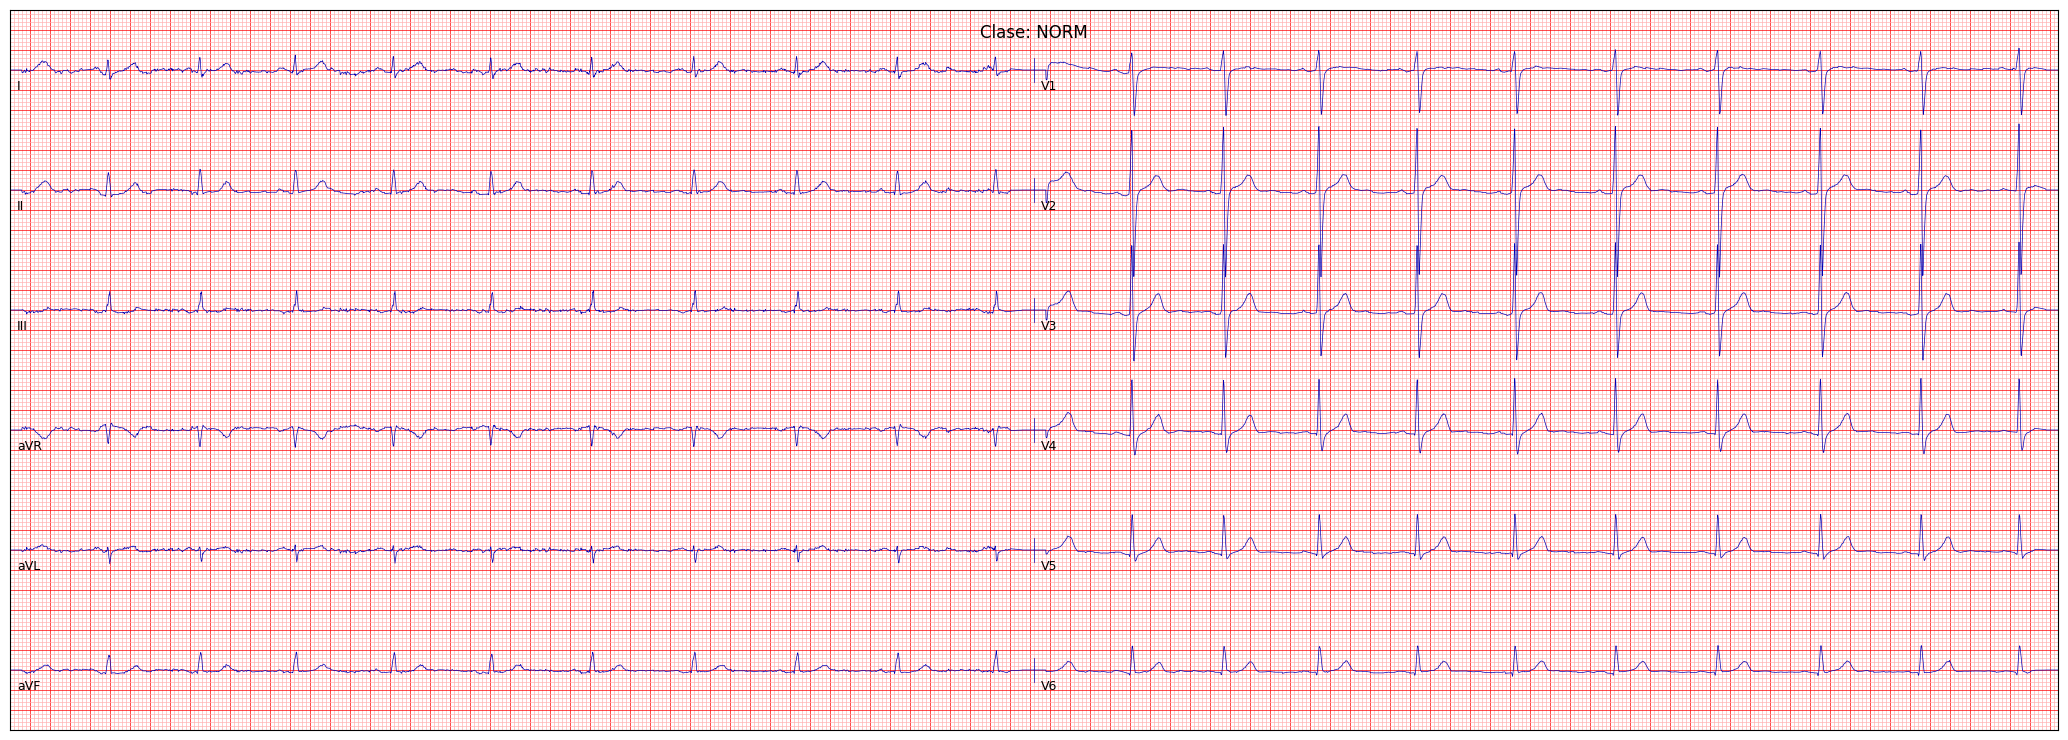
\includegraphics[width=0.9\textwidth]{Imagenes/Vectorial/ECG/NORM.png}
	 	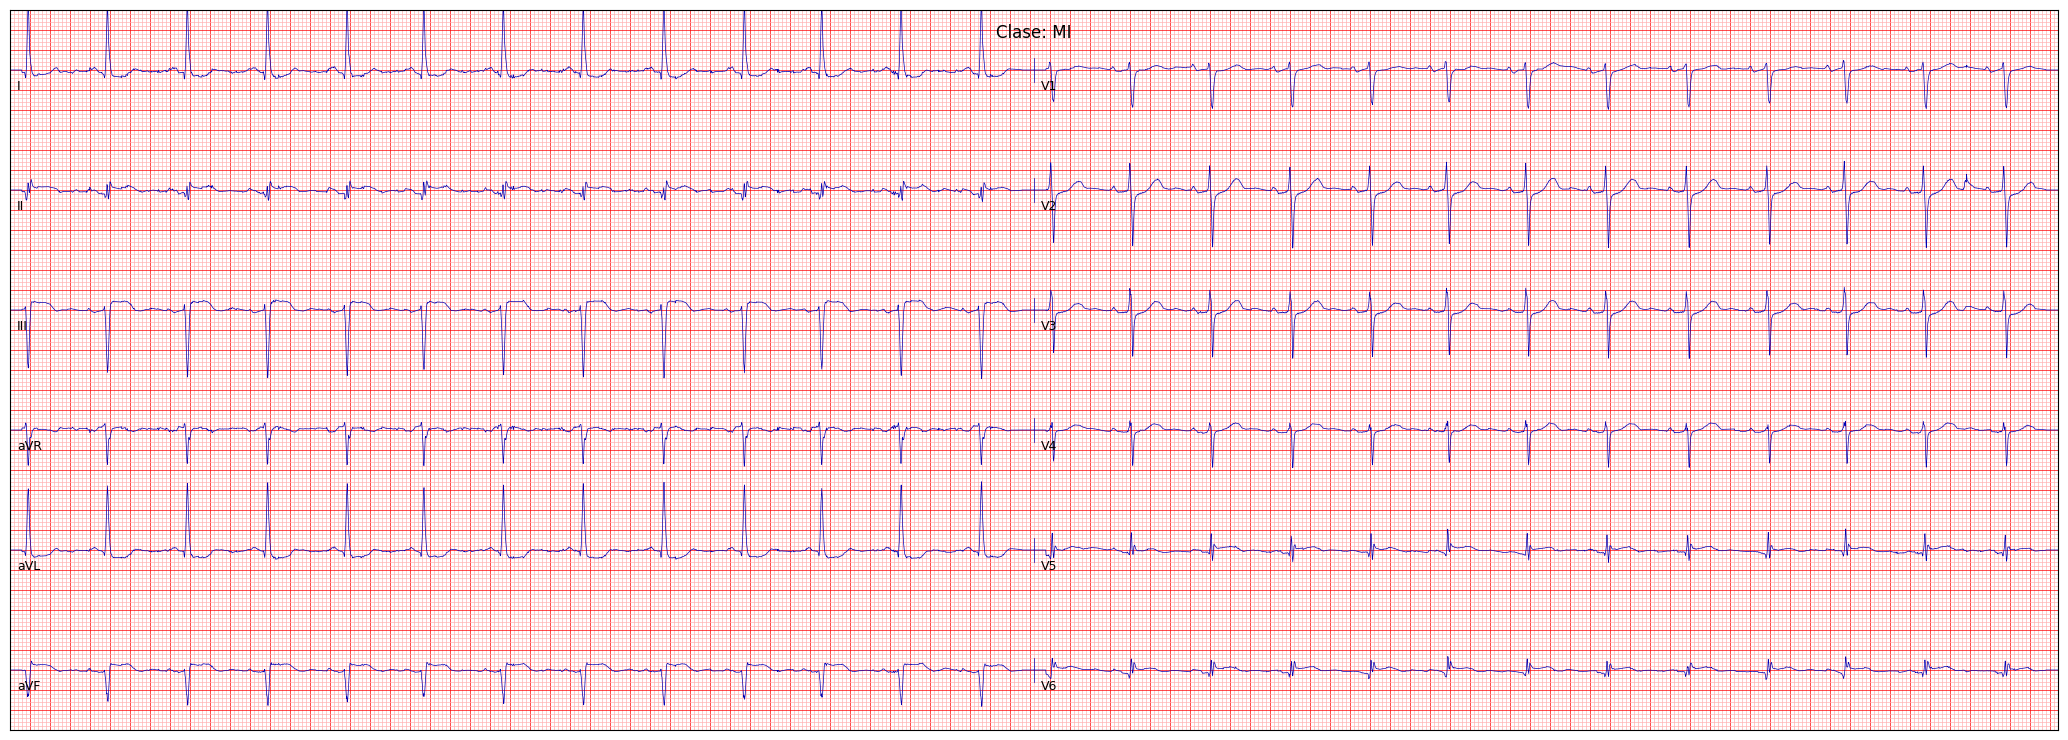
\includegraphics[width=0.9\textwidth]{Imagenes/Vectorial/ECG/MI.png}
	 	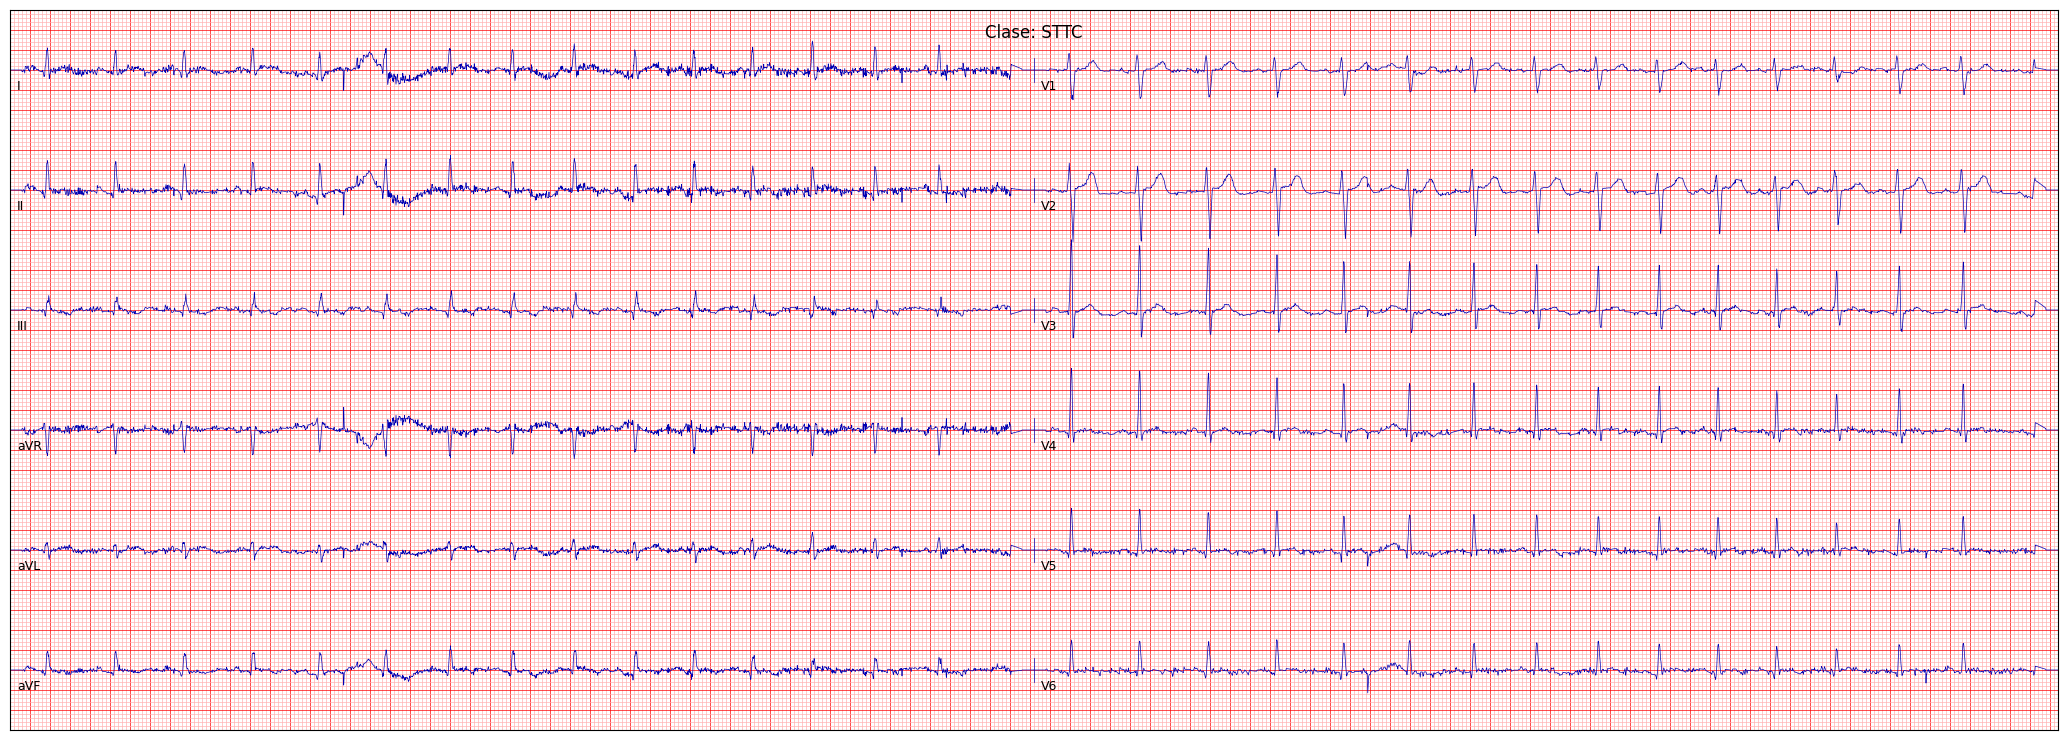
\includegraphics[width=0.9\textwidth]{Imagenes/Vectorial/ECG/STTC.png}
	 	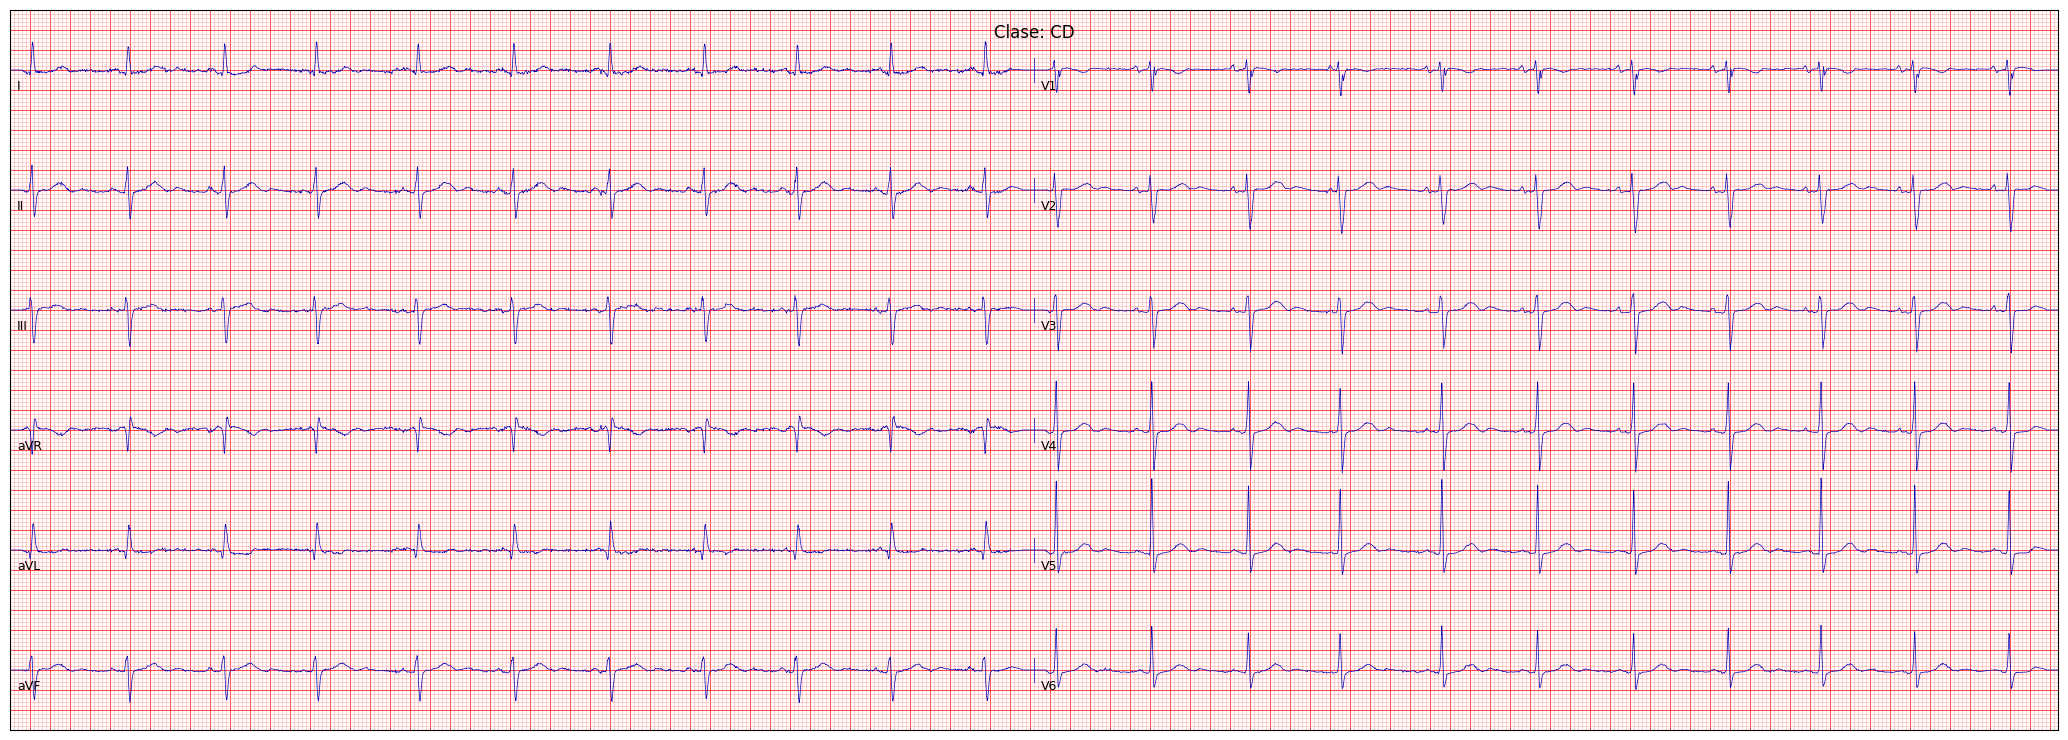
\includegraphics[width=0.9\textwidth]{Imagenes/Vectorial/ECG/CD.png}
	 	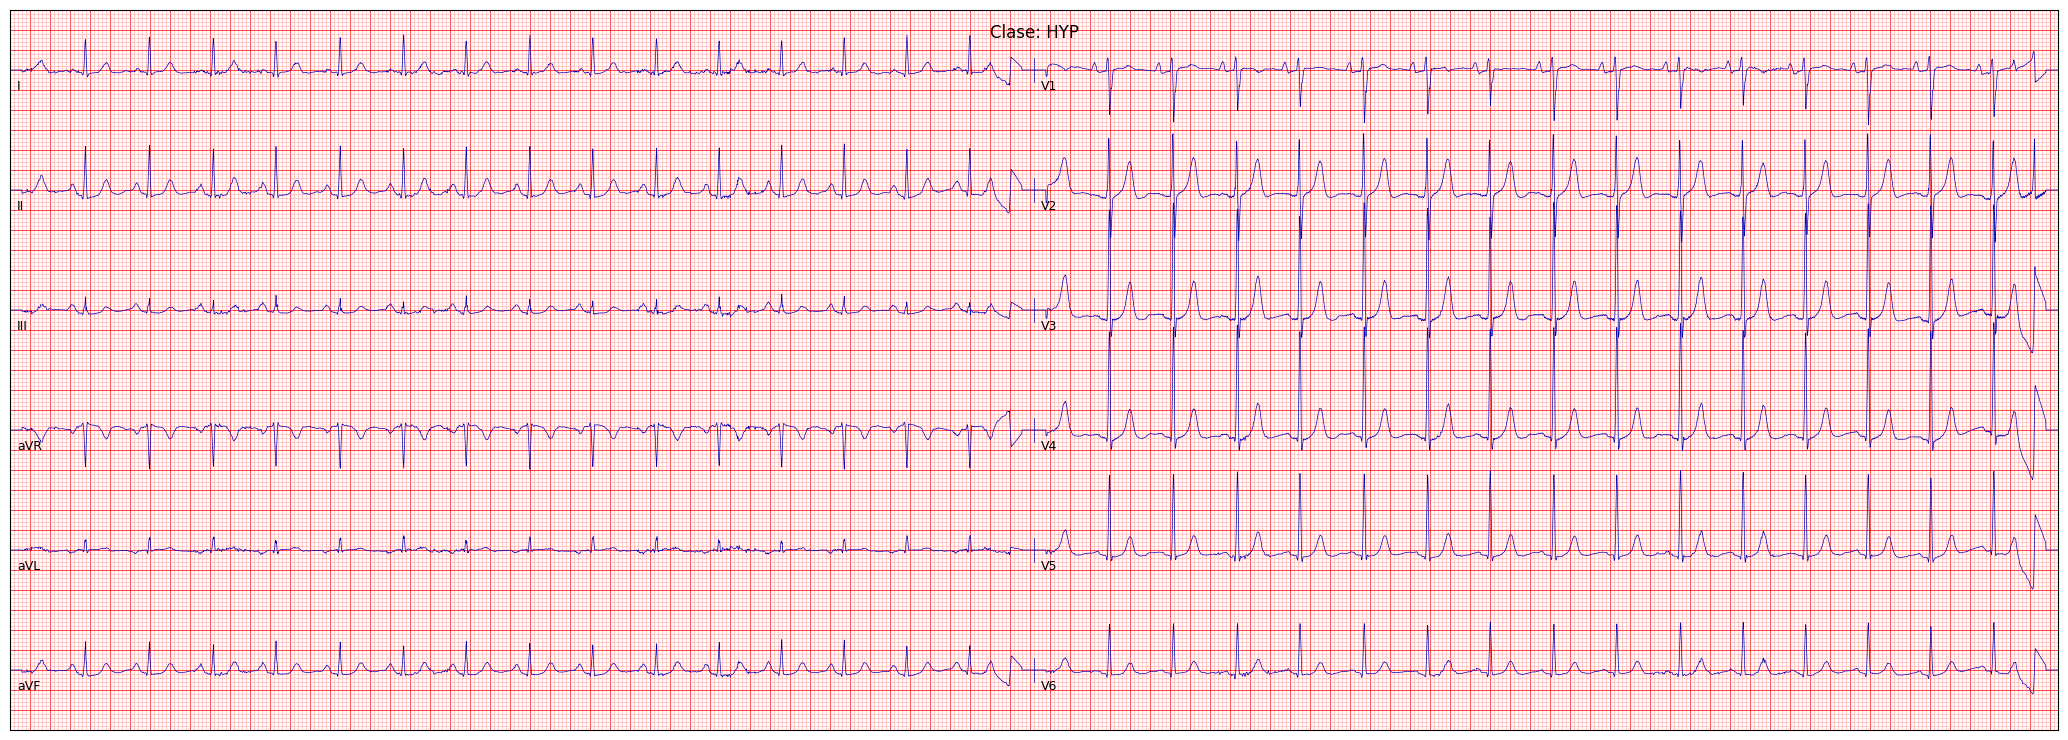
\includegraphics[width=0.9\textwidth]{Imagenes/Vectorial/ECG/HYP.png}
	 	\caption{ECGs de todos los tipos de anomalías.}
	 	\label{fig:ecg_clases}
	 \end{figure}
	
	\subsubsection{Formato de los datos}
	Los ECGs se almacenan en formato WFDB (\emph{Waveform Database}), un estándar ampliamente utilizado en el ámbito médico para almacenar datos de señales anotados \citep{wfdb_spec}.
	
	\subsubsection{Información de pacientes}
	Cada ECG está asociado a información demográfica (edad, sexo, etc.)

En este trabajo únicamente tendremos en cuenta las doce derivaciones del ECG, así como las anotaciones que permiten clasificarlo en una de las cinco etiquetas contempladas en la Sección \ref{subsec:anomalias}.

\section{Modelos para la clasificación de ECG}
\subsection{Enfoques basados en técnicas tradicionales de aprendizaje automático}
El desarrollo de clasificadores ha sido crucial en el campo de la IA enfocada a la detección de anomalías en señales de ECGs. Entre estos métodos, los árboles de decisión y el método k-NN han mostrado una eficiencia notable gracias a su sencillez y capacidad para modelar comportamientos complejos \citep{guo2023machine}.

No obstante, estos enfoques presentan un problema, pues requieren seleccionar de manera manual una serie de características en la señal (como amplitud de la onda R, duración del complejo QRS, etc.), cosa que resulta extremadamente difícil ya que el análisis de electrocardiogramas es muy complejo. Aunque estos métodos resultan efectivos en escenarios con un volumen de datos moderado, su rendimiento depende en gran medida de las características anteriormente mencionadas \citep{acharya_2017}.

\subsection{Modelos basados en redes neuronales}
Las redes neuronales son un modelo computacional inspirado en las neuronas biológicas. Están formadas por capas de neuronas artificiales conectadas entre sí que aprenden a transformar los datos de las entradas en las salidas deseadas. Este aprendizaje se realiza ajustando los pesos de cada conexión, comúnmente mediante el algoritmo de \emph{backpropagation} \citep{backpropagation}, para minimizar un error definido (p.ej., la diferencia entre la salida prevista y la real). De esta forma, en lugar de depender de técnicas de extracción de características diseñadas manualmente, las redes neuronales aprenden internamente los rasgos más relevantes a partir de los datos.

En particular, las CNNs (\emph{Convolutional Neural Networks}, Redes Neuronales Convolucionales) se han popularizado en tareas de visión por computador y análisis de señales al emplear operaciones de convolución (ver siguiente apartado).

Aunque nacieron enfocadas al reconocimiento de imágenes, se han adaptado con éxito a otros tipos de datos, como ondas, usando convoluciones unidimensionales en lugar de bidimensionales. Esto permite a la red detectar características relevantes de la señal (como la forma o duración de los intervalos) sin necesidad de ser elegidas manualmente por un experto, lo que le otorga una gran capacidad de generalización \citep{hannun_cardiologist_2019}.

\subsubsection{Convoluciones}
Una convolución es una operación matemática que toma dos funciones o señales y produce una tercera, mostrando cómo una de ellas “filtra” a la otra. Por ejemplo, en el procesamiento de imágenes, la convolución se utiliza para aplicar filtros o detectores de bordes: se toma una matriz de píxeles (la imagen) y se combina con un kernel (también llamado filtro), multiplicando y sumando los valores de cada posición para generar un nuevo valor en la imagen resultante. Este proceso, repetido a lo largo de toda la matriz, ayuda a resaltar características como contornos o texturas específicas.

En redes neuronales, se utilizan convoluciones discretas (es decir, diseñadas para trabajar con una cantidad de datos discreta, lo que ocurre siempre ya que los datos son finitos) .La convolución es la base para extraer características relevantes de datos de entrada como imágenes o señales (como es el caso de un ECG). Cada capa convolucional aprende pesos que responden a cierto patrón, de modo que, al aplicar esa capa sobre la entrada, se pueden detectar patrones específicos (por ejemplo, la presencia de bordes horizontales o verticales en una imagen). A través de varias capas de convolución, el modelo va construyendo representaciones cada vez más complejas, y eso permite un gran en tareas de clasificación (como es el caso de los ECGs). Esta eficiencia y capacidad de extracción de características es lo que ha convertido a las convoluciones en una herramienta fundamental dentro de la informática moderna, especialmente en los campos de visión por computadora.

\subsection{El modelo de Ribeiro}
Dentro de los enfoques basados en redes convolucionales, destaca el modelo propuesto por \cite{ribeiro}, cuyo objetivo es la clasificación multiclase de ECGs de 12 derivaciones. La arquitectura (que podemos ver en la Figura \ref{fig:ribeiro_arch}) se caracteriza por una serie de capas convolucionales unidimensionales adaptadas a la naturaleza de la señal. Esto permite analizar el electrocardiograma como una señal, sin necesidad de representarla como una imagen.

\begin{figure}[t]
	\centering
	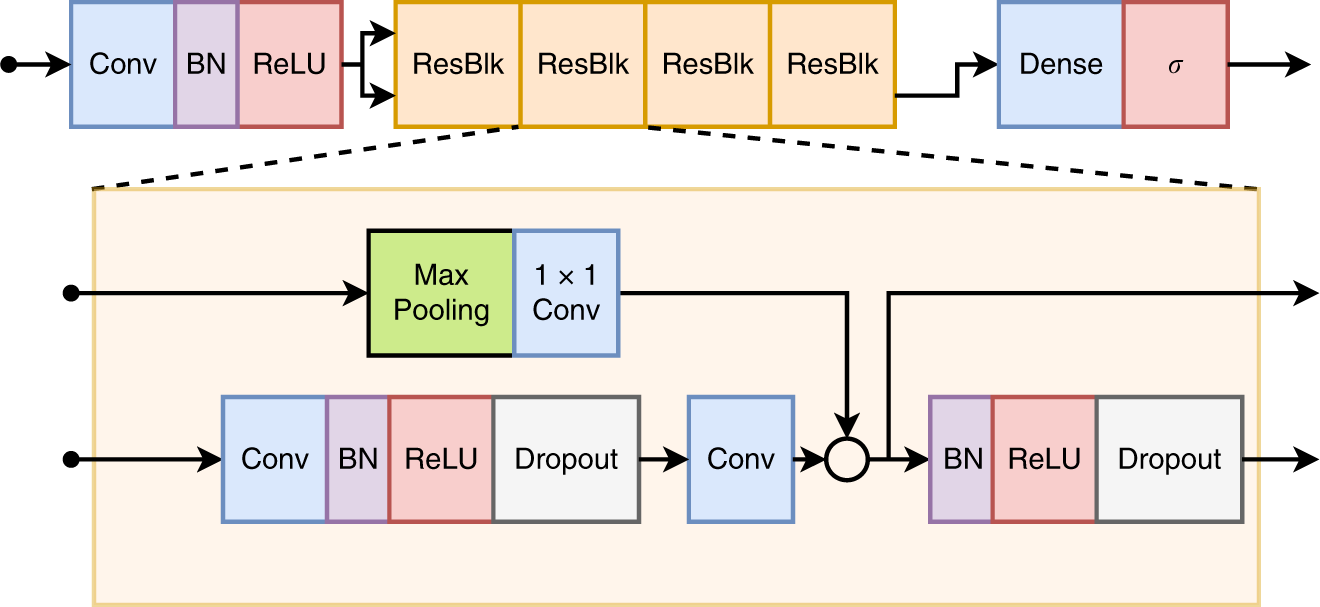
\includegraphics[width=\textwidth]{Imagenes/Vectorial/ribeiro_arch.png}
	\caption{Arquitectura de la red neuronal que se emplea en el \emph{gold standard}. Fuente: \cite{ribeiro}}
	\label{fig:ribeiro_arch}
\end{figure}

Los distintos tipos de capas que utiliza el modelo son las siguientes (para ver más sobre los tipos de capas y su comportamiento completo, el lector puede referirse a \textbf{Deep Learning} \cite{Goodfellow-et-al-2016}):

\begin{enumerate}
	\item \textbf{Conv}: Las capas convolucionales mencionadas anteriormente.
	\item  \textbf{BN}: Son capas de \emph{batch normalization}, que mejoran y aceleran el entrenamiento.
	\item \textbf{ReLU}: Capas de activación, que devuelven 0 si el valor de la entrada es negativo.
	\item \textbf{Dropout}: Una capa que desactiva un porcentaje aleatorio de las neuronas en cada entrenamiento, para evitar ciertos problemas como la sobrespecialización.
	\item \textbf{Max Pooling}: Se utiliza para reducir la dimensionalidad de la entradda.
	\item \textbf{Dense}: Esta capa se suele utilizar antes de una función de activación para adecuar el número de salidas del problema
	\item \textbf{$\sigma$}: Capas sigmoides, transforman la salida de las neuronas en un valor real entre 0 y 1. Son útiles para acotar la salida.
\end{enumerate}

Como puede verse en el artículo de \cite{ribeiro}, el modelo demostró un alto desempeño en la detección de diversas anomalías. En este trabajo, adaptaremos ligeramente la capa de entrada de este modelo para poder tomar como entrada matrices de cualquier tamaño (originalmente el modelo requería de matrices de dimensión 12xN) para poder entrenarlo con transformaciones de la señal original a imágenes. Sin embargo, no modificaremos la estructura interna de las capas convolucionales.

\section{Explicabilidad en la IA}
A pesar de que los modelos de \emph{Deep Learning} han demostrado su eficacia en tareas de diagnóstico clínico, es necesario contar con métodos que ofrezcan explicaciones y permitan interpretar sus predicciones, ya que la actual legislación europea (\href{https://europa.eu/youreurope/business/dealing-with-customers/data-protection/data-protection-gdpr/index_es.htm}{\emph{GDPR}}) exige poder dar una explicación comprensible de cualquier decisión tomada por un algoritmo o modelo predictivo. Esto es particularmente relevante en el ámbito médico, donde cualquier decisión que tome un algoritmo debe poder justificarse ante profesionales de la salud, ya que la salud de una persona podría verse afectada por esta decisión.

Algunos de los métodos más notables de explicación en la IA son los siguientes:

\subsubsection{Métodos intrínsecos}
Estos métodos consisten en analizar el código del modelo de IA para comprender qué hace exactamente un modelo por dentro. Estos métodos solo son aplicables cuándo el el modelo es intrínsecamente explicable, es decir, que hay una clara correlación entre el código del modelo y la salida del mismo, como es el caso de los árboles de decisión o regresiones lineales.

Las redes neuronales no entran dentro de este tipo de modelos, y por tanto no podemos aplicar este tipo de explicaciones en este trabajo.

\subsubsection{Métodos basados en visualización}
Estos métodos consisten en representar gráficamente qué partes de la entrada son más relevantes a la hora de tomar una decisión. Por esto, están estrechamente relacionados con el significado de los datos de entrada, y no tanto con su forma. Supongamos que tenemos como entrada una matriz de dos dimensiones. Esto puede interpretarse (entre otras cosas) como una imagen o como una serie de vectores de mediciones distintas (esto último se conoce como serie temporal) en el tiempo:

\begin{itemize}
	\item Si los datos representan imágenes, existen métodos como Grad-CAM para dibujar mapas de calor sobre la imagen original que señalan las partes más relevantes de la imagen a la hora de tomar decisiones.
	\item Si tenemos una serie temporal, para explicar qué zonas son más importantes lo que necesitamos es señalar, en cada una de las mediciones, qué franjas temporales son más relevantes para la decisión. Esto es lo que hacen algunos métodos como \emph{saliency maps}.
\end{itemize}

\par

Si bien es cierto que en este trabajo tenemos tanto series temporales (los datos originales sin transformar) como imágenes (los datos transformados), en este trabajo utilizaremos exclusivamente \emph{saliency maps}, por motivos que veremos en el Capítulo \ref{cap:explicabilidad}.


\chapter{Metodología y preparación de datos}
\label{cap:pre_datos}
\begin{resumen}
	En este capítulo describimos la metodología seguida para procesar y transformar las señales de ECG de la base de datos PTB-XL, detallamos la distribución de las clases, el preprocesamiento aplicado, las transformaciones realizadas y las métricas empleadas para evaluar los modelos.
\end{resumen}

\section{Análisis de los datos y distribución por clases}
La base de datos PTB-XL es un conjunto de registros formado por 21799 ECGs de 12 derivaciones, considerado uno de los mayores \emph{datasets} públicos de ECGs disponibles en la actualidad \citep{ptbxlart}. Contiene muestras de ECGs de 10 segundos de duración anotadas con múltiples etiquetas diagnósticas. Para este trabajo, emplearemos la clasificación según las superclases definidas en la propia base de datos, que coinciden con las que presentamos en la Sección \ref{subsec:anomalias}.

La Tabla \ref{tab:dist} muestra la distribución de los datos de PTB-XL considerando estas cinco superclases. Se observa que la clase ``NORM'' es la más numerosa, mientras que la clase ``HYP'' tiene una cantidad considerablemente menor de datos. Este desbalanceo de clases puede causar varios problemas en el modelo, como por ejemplo:

\begin{table}[t]
	\centering
	\begin{tabular}{|lllr|}
		\hline
		Número de registros & Superclase & Descripción & Porcentaje \\
		\hline
		9514 & NORM & ECG Normal & 43.64\% \\
		5469 & MI & Infarto de Miocardio & 25.08\% \\
		5235 & STTC & Cambio ST/T & 24.01\% \\
		4898 & CD & Transtorno de la conducción & 22.46\% \\
		2649 & HYP & Hipertrofia & 12.15\% \\
		\hline
		
	\end{tabular}
	\caption{Distribución de las superclases en PTB-XL}
	\label{tab:dist}
	\begin{tablenotes}
		\small
		\item La información de esta tabla ha sido extraída directamente del \href{https://physionet.org/content/ptb-xl/1.0.3/}{repositorio de PTB-XL}.
	\end{tablenotes}
\end{table}

\begin{enumerate}
	\item \textbf{Sobreajuste hacia la clase mayoritaria:} Al haber bastantes más datos de entrenamiento de una clase (NORM) y menos de otra (HYP), el modelo puede aprender mejor los patrones que identifican las clases mayoritarias, haciendo que sepa distinguir peor las minoritarias, lo que en este caso podría reducir notablemente su capacidad de predicción de anomalías raras \citep{IData}.
	
	\item \textbf{Métricas no representativas:} Las métricas más comunes, como la exactitud, pueden ser poco informativas cuando hay un desbalance en los datos de prueba, ya que un modelo que predice siempre la clase mayoritaria puede tener una exactitud alta. Esto puede dificultar la evaluación real del rendimiento del modelo \citep{ClassOfIData}.
	
	\item \textbf{Dificultad en el entrenamiento:} Las redes neuronales profundas requieren de grandes cantidades de datos de entrenamiento para poder entender patrones complejos. Si una de las clases tiene muy pocos ejemplos, es muy probable que el modelo no sea capaz de predecirla correctamente \citep{Leevy}.
\end{enumerate}

Para abordar estos problemas existen varias estrategias, como hacer \emph{oversampling} o \emph{undersampling}. El \emph{oversampling} consiste en generar datos sintéticos a partir de los que ya tenemos para balancear las clases \citep{he2008adasyn}, pero esto no es una buena técnica cuándo los datos son complejos (como es el caso de un electrocardiograma), ya que no hay una técnica clara para crear datos sintéticos coherentes. Por otro lado, el \emph{undersampling} hace que todas las clases se queden con el mismo número de candidatos que la clase minoritaria, lo que no es una técnica adecuada cuándo los datos de entrenamiento son reducidos desde un principio \citep{koziarski2019radial}.

\section{Preprocesamiento de datos}
\label{sec:procesamiento}
En cualquier desarrollo de IA, antes de poder utilizar los datos hay que hacer cierto procesamiento para asegurarnos que son adecuados. Lo primero que habría que hacer es quitar los datos repetidos, incompletos o corruptos, pero afortunadamente la base de datos que estamos utilizando ya ha sido revisada por sus creadores, por lo que podemos obviar este paso.

En procesamiento de señales biomédicas (especialmente en señales que son muy sensibles a determinadas perturbaciones, como es el caso de los ECGs) es muy importante aplicar determinados filtros antes de trabajar con las señales. En este trabajo utilizaremos los scripts que se utilizaron en el trabajo de \cite{TFGSergio} (que nos han sido facilitados por el autor y están basados en el trabajo original de \cite{ribeiro}). En concreto, los datos se preprocesan de la siguiente manera:
\begin{itemize}
	\item Se reescalan todos para tener una frecuencia de 400Hz, que es con la que se entrenó al \emph{gold standard}. Por tanto, tras hacer este procesamiento previo estaremos trabajando con vectores de 4096 elementos.
	\item Se elimina el desplazamiento de la línea base, que son las interferencias de baja frecuencia generadas por la respiración. Como podemos ver en \cite{baseline}, es muy importante hacer esto antes de analizar un ECG.
	\item Se elimina la interferencia de la línea de alimentación, que es l a interferencia generada por la corriente eléctrica del aparato medidor, lo que también es importante como podemos ver en \cite{powerline}.
\end{itemize}

Por último, separamos los datos en tres conjuntos. Los autores de la base de datos presentan una estratificación (es decir, una división equilibrada de los datos) en diez clases (numeradas del uno al diez), y recomiendan utilizar el noveno estrato para validación, el décimo para pruebas y el resto para entrenamiento. Siguiendo esa clasificación, tendremos los siguientes conjuntos:
\begin{itemize}
	\item \textbf{Entrenamiento (\emph{train}):} El conjunto mayoritario (con un 80\% de los datos, es decir 17418 casos), que será usado para entrenar al modelo.
	\item \textbf{Validación (\emph{validation}):} Este conjunto (que representa el 10\% de los datos, es decir 2183) se utilizará para ajustar los parámetros del modelo en el entrenamiento del mismo.
	\item \textbf{Pruebas (\emph{test}):} Este conjunto (que está formado por el 10\% restante de los datos, es decir 2198 casos) es el que utilizaremos para obtener las diversas métricas de rendimiento del modelo.
\end{itemize}

\section{Métricas de evaluación}
En este apartado revisamos algunas de las métricas típicamente utilizadas y que usaremos para evaluar nuestros modelos.

\subsection{Métricas habituales}
Entre las métricas más habituales podemos encontrar la \emph{F-$\beta$ Score}, \emph{precision} y \emph{recall}.

\subsubsection{Precision (Precisión)}
La precisión es la proporción de predicciones positivas que son realmente positivas, o más concretamente:
\[
\text{Precision} = \frac{\text{Verdaderos positivos}}{\text{Verdaderos positivos + Falsos positivos}}.
\]

Un valor alto de esta métrica indica que el modelo es bueno minimizando falsos positivos, es decir, cuándo el modelo predice que un dato no pertenece a una clase, esa predicción es fiable.

\subsubsection{Recall (Sensibilidad)}
La sensibilidad mide la proporción de casos positivos que el modelo predice correctamente, o más concretamente:
\[
\text{Recall} = \frac{\text{Verdaderos positivos}}{\text{Verdaderos positivos + Falsos negativos}}.
\]

Un valor alto de esta métrica indica que el modelo es bueno minimizando falsos positivos, es decir, cuándo el modelo predice que un dato pertenece a una clase, esa predicción es fiable.

\subsubsection{F-$\beta$ Score}
El F-$\beta$ Score es una media entre la precisión y el recall, la fórmula concreta es:
\[
F_\beta = (1+\beta^2)\times \frac{\text{precision} \times \text{recall}}{\beta^2\times\text{precision} + \text{recall}}.
\]
El valor más habitual para esto es $\beta=1$, que nos da la media armónica y permite valorar tanto la fiabilidad del modelo cuando predice positivo como negativo.

Esto es adecuado cuándo, por la naturaleza de un problema, el coste de los falsos positivos es similar al de los falsos negativos, pero no es nuestro caso. En modelos aplicados a la salud, es mucho más importante predecir las anomalías correctamente (ya que de esto puede depender la salud de una persona) que predecir correctamente la ausencia de anomalías.

Los valores de $\beta=0.5$ y $2$ hacen que tenga más peso la precisión y el recall respectivamente, por lo que la primera es más adecuada para cuándo los falsos positivos tienen un coste muy alto y la segunda para cuándo son los falsos negativos los que tienen el coste más alto.

\subsection{Métricas en clasificadores multietiqueta}
Todas las métricas que hemos listado anteriormente están definidas para clasificadores binarios, pero nuestro clasificador es multietiqueta, por lo que es necesario adaptarlas. Tres de los enfoques más habituales a este problema son el cálculo por clases, el promedio binario y el \emph{micro average}.

\subsubsection{Cálculo por clase}
Este es el enfoque más sencillo de todos. Consideramos nuestro clasificador multietiqueta como uno binario para cada una de sus etiquetas, y calculamos las métricas para cada una de las clases.

Este enfoque permite ver el desempeño del modelo en cada una de sus clases, lo que permite entender mejor cuáles son sus debilidades y fortalezas. El principal problema que presenta este método es que no da un único valor para comparar modelos, por lo que puede ser difícil determinar qué modelo es el óptimo.

\subsubsection{Promedio binario}
El promedio binario (también conocido como \emph{one-vs-rest}) consiste en tratar cada clase de forma independiente frente a las demás, calcular las métricas para cada clase de manera binaria y, finalmente, promediarlas. De este modo, cada clase se considera positivamente etiquetada en un escenario (con sus correspondientes verdaderos positivos, falsos positivos y falsos negativos) mientras que el resto de las clases se consideran negativamente etiquetadas.

Este método permite obtener un valor global de la métrica (por ejemplo, F1) que resume el desempeño del modelo en todas las clases, pero puede enmascarar diferencias importantes en la distribución de datos (por ejemplo, cuando el número de instancias de cada clase es muy desigual). Sin embargo, sigue siendo un enfoque útil si se desea una única medida para comparar el rendimiento de diferentes clasificadores. 


\subsubsection{\emph{Micro average}}
El \emph{micro average} se basa en sumar las predicciones correctas e incorrectas de todas las clases antes de calcular las métricas. En lugar de promediar los resultados clase por clase, este método reúne todos los verdaderos positivos, falsos positivos y falsos negativos de manera global. A continuación, se calcula la métrica global a partir de estos valores agregados.

Esta aproximación proporciona un único valor general de desempeño del modelo, especialmente útil cuando se desea obtener una medida global en problemas de múltiples clases o etiquetas. El micro average, al considerar todos los ejemplos de forma conjunta, puede ofrecer una visión más equilibrada del rendimiento global, aunque a costa de no mostrar el detalle de cómo se comporta el modelo en cada clase individual. 


\subsection{Métricas para nuestro problema}
Tras realizar el análisis de las posibles métricas que implementar, hemos decidido calcular y mostrar varias métricas para cada modelo, y elegir una que consideramos mejor para afirmar qué modelo es el mejor. Para hacer métricas globales, ya que nuestros datos presentan un importante desbalanceo en una de sus clases, utilizaremos \emph{micro average}. Las métricas que mostraremos son las siguientes:

\begin{itemize}
	\item Para cada una de las clases:
	\begin{itemize}
		\item Precisión.
		\item Recall.
		\item F-1 Score.
	\end{itemize}
	\item Precisión global calculada como \emph{micro average}.
	\item Recall global calculado como \emph{micro average}.
	\item F-1 Score global calculado como \emph{micro average}.
	\item F Score ajustada, una métrica personalizada que definiremos a continuación.
\end{itemize}

Todas las métricas que mostraremos, salvo la personalizada, tienen el objetivo de entender mejor cómo funciona el modelo, no obstante, es útil escoger una sola métrica para poder comparar estrictamente qué modelo consideramos \emph{mejor}. Esta métrica será la F Score ajustada 

Dado que nuestro modelo es un clasificador en el que las etiquetas no tienen el mismo significado, ya que una de ellas representa un ECG normal mientras que las demás representan diversas anomalías, el coste de los falsos positivos o negativos varía dependiendo de la etiqueta. Nuestro objetivo es que el modelo identifique lo mejor posible las anomalías (cuándo las haya), por lo que el coste de los falsos negativos en las etiquetas de anomalías es muy alto, mientras que el coste de los falsos positivos en la etiqueta normal es muy alto.

Por ello, definiremos la F Score ajustada como la media de la F-0.5 Score de la clase normal y las  F-2 Score del resto de etiquetas. Esto nos permite tener una métrica que tiene en cuenta tanto reducir falsos negativos como falsos positivos en todas las etiquetas, pero dando más peso a los falsos negativos o positivos dependiendo de la etiqueta concreta.

La fórmula concreta de la métrica sería:
\begin{equation*}
	\text{F Score ajustada} = \frac{F-0.5(\text{NORM}) + \sum_{i \neq \text{NORM}}F-2(i)}{\text{Número de clases}}
\end{equation*}


\section{Transformaciones}

Pueden aplicarse gran cantidad de transformaciones a una señal antes de procesarla. En nuestro caso concreto, aplicamos una transformada STFT y otra CWT, ambas en sus versiones discretas. En las siguientes secciones explicaremos la idea general de estas transformadas. Para una definición formal de estas, así como un estudio más detallado de sus propiedades y aplicaciones, pueden consultarse \cite{Oppenheim2009, Allen1977}.

\subsection{STFT}
\label{subsec:stft}

La Transformada de Foutier en Tiempo Corto (STFT, del inglés \emph{Short-Time Fourier Transform}) es una herramienta matemática utilizada para analizar la evolución espectral de una señal a lo largo del tiempo. A diferencia de la Transformada de Fourier convencional, que proporciona información global sobre la distribución de las frecuencias de una señal sin preservar la dimensión temporal, la STFT incorpora una ventana que permite observar cómo las frecuencias van cambiando localmente en el tiempo \citep{Allen1977, Oppenheim2009}.

En nuestro contexto, la STFT resulta particularmente útil porque permite estudiar señales no estacionarias, es decir, aquellas cuyas características cambian a lo largo del tiempo. El ECG es un ejemplo de este tipo de señal, ya que su frecuencia varía debido factores como cambios en el ritmo, arritmias u otras alteraciones.

La STFT divide la señal en pequeños segmentos de tiempo (llamados ventanas) y aplica la Transformada de Fourier a cada uno de ellos, lo que permite obtener una representación en el dominio tiempo-frecuencia. Esto significa que podemos visualizar cómo cambian las diferentes frecuencias de la señal en el tiempo.

Esta capacidad de analizar variaciones temporales de la frecuencia hace que la STFT sea ideal para identificar eventos transitorios en el ECG, como la aparición repentina de una arritmia, alteraciones momentáneas en la forma de las ondas, o cambios en la frecuencia cardíaca, que suelen indicar anomalías médicas como las que estamos intentando detectar.

A la hora de implementar la STFT, existen varios parámetros importantes a ajustar:

\begin{itemize}
	\item \textbf{Ventana (\emph{window})}: Se utiliza una ventana de tipo Hann. La ventana Hann es una función que reduce el efecto de discontinuidades en los bordes del segmento.
	
	\item \textbf{Frecuencia de muestreo}: La señal original se encuentra muestreada a 400 Hz. Esta frecuencia de muestreo determina la resolución temporal que se logra.
	
	\item \textbf{Longitud del segmento}: Se utilizan 256 muestras. El segmento de datos tomado para cada ventana afecta la resolución en frecuencia. Un mayor número de puntos mejora la resolución en frecuencia, pero empeora la resolución temporal.
	
	\item \textbf{Solapamiento}: Se emplea 128 muestras. Esto significa que cada ventana se solapa con la mitad (128 muestras) de la ventana anterior. Un solapamiento mayor permite detectar eventos transitorios con mayor detalle temporal, a costa de un mayor costo computacional.
	
\end{itemize}

La elección de estos parámetros busca un equilibrio entre la resolución temporal y frecuencial, adecuado para el análisis de señales cardíacas. El tamaño de 256 muestras por segmento, junto con la frecuencia de muestreo de 400 Hz, ofrece una resolución en frecuencia suficiente para el rango de interés cardiológico; y el solapamiento de 128 muestras asegura una adecuada continuidad y capacidad de capturar eventos transitorios.

En la Figura \ref{fig:stft} se presenta un ejemplo de la transformada STFT aplicada a la primera derivación de un ECG de cada clase diagnóstica con los parámetros que acabamos de elegir. La representación muestra cómo las frecuencias varían en función del tiempo, lo que permite ver eventos específicos como arritmias o cambios en las características de las ondas. Esta visualización puede ayudar a comprender y analizar los patrones complejos presentes en las señales del ECG.

\begin{figure}[t]
	\centering
	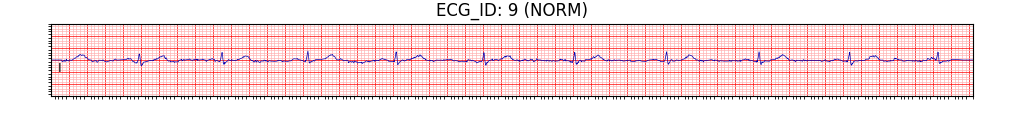
\includegraphics[width=0.95\textwidth]{Imagenes/Vectorial/Transformadas/NORM/ecg.png}
	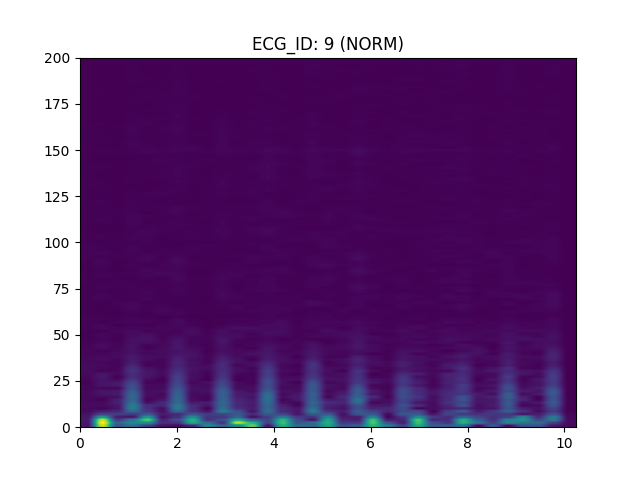
\includegraphics[width=0.45\textwidth]{Imagenes/Vectorial/Transformadas/NORM/stft.png}
	\par Primera derivación de un ECG normal (arriba) y su transformada STFT (abajo).
	\vspace{1cm}
	
	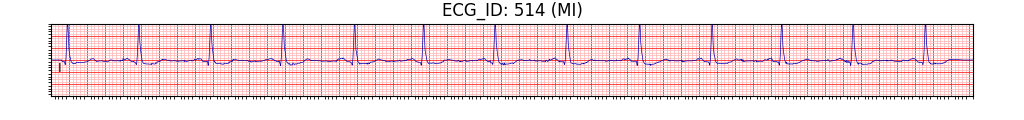
\includegraphics[width=0.95\textwidth]{Imagenes/Vectorial/Transformadas/MI/ecg.png}
	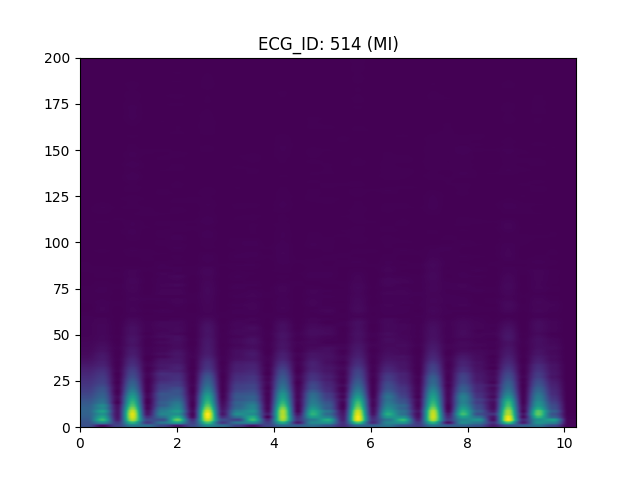
\includegraphics[width=0.45\textwidth]{Imagenes/Vectorial/Transformadas/MI/stft.png}
	\par Primera derivación de un ECG de infarto de miocardio (arriba) y su transformada STFT (abajo).
	\caption{Transformadas STFT de la primera derivación de ECGs para cada clase.}
	\label{fig:stft}
\end{figure}
\begin{figure}[t]\ContinuedFloat
	\centering
	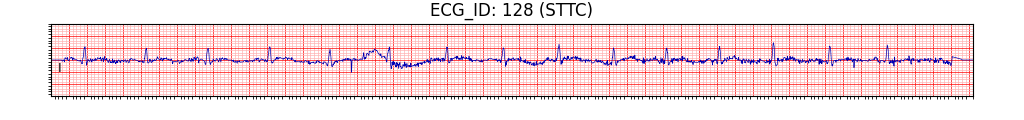
\includegraphics[width=0.95\textwidth]{Imagenes/Vectorial/Transformadas/STTC/ecg.png}
	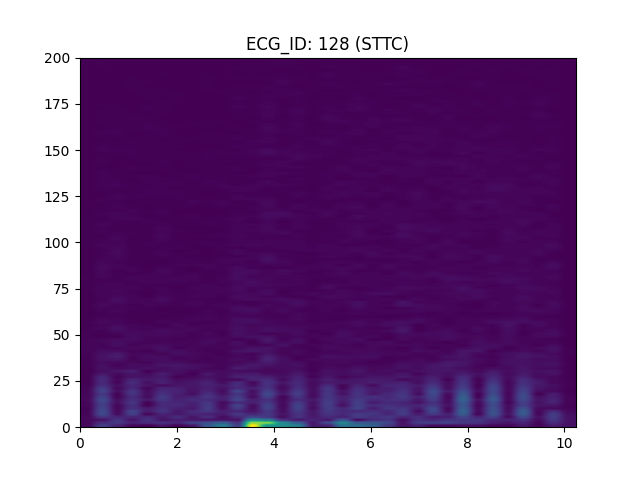
\includegraphics[width=0.45\textwidth]{Imagenes/Vectorial/Transformadas/STTC/stft.png}
	\par Primera derivación de un ECG de tipo STTC (arriba) y su transformada STFT (abajo).
	\vspace{1cm}
		
	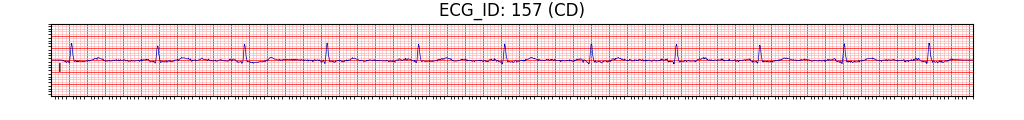
\includegraphics[width=0.95\textwidth]{Imagenes/Vectorial/Transformadas/CD/ecg.png}
	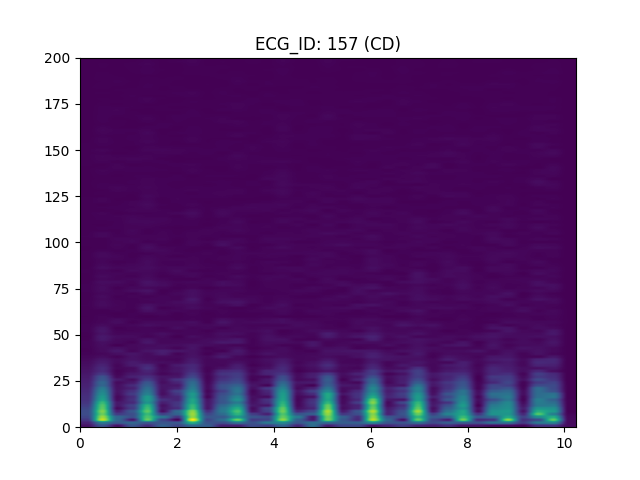
\includegraphics[width=0.45\textwidth]{Imagenes/Vectorial/Transformadas/CD/stft.png}
	\par Primera derivación de un ECG de tipo CD (arriba) y su transformada STFT (abajo).
	\caption{Transformadas STFT de la primera derivación de ECGs para cada clase.}
\end{figure}
\begin{figure}[t]\ContinuedFloat
	\centering
	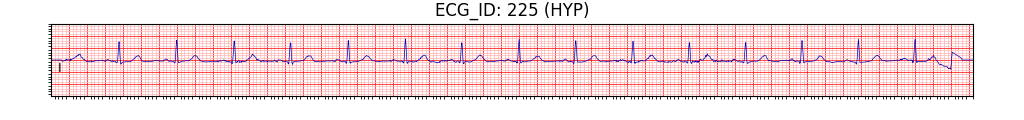
\includegraphics[width=0.95\textwidth]{Imagenes/Vectorial/Transformadas/HYP/ecg.png}
	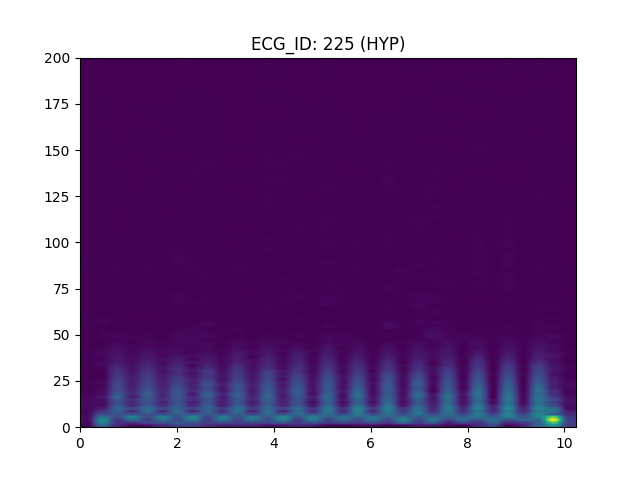
\includegraphics[width=0.45\textwidth]{Imagenes/Vectorial/Transformadas/HYP/stft.png}
	\par Primera derivación de un ECG con hipertrofia (arriba) y su transformada STFT (abajo).
	\caption{Transformadas STFT de la primera derivación de ECGs para cada clase.}
\end{figure}

\subsection{CWT}
\label{subsec:cwt}
La Transformada de Onda Continua (CWT, del inglés \emph{Continous Wavelet Transform}) es una técnica matemática utilizada para analizar señales no estacionarias. A diferencia de la Transformada de Fourier, la CWT descompone la señal en funciones llamadas \emph{wavelets}, que se representan en función de tiempo-frecuencia. Esto (al igual que con la STFT) permite una mayor precisión al estudiar eventos transitorios, ya que las \emph{wavelets} pueden ajustarse para capturar detalles de diferentes escalas temporales o frecuenciales.

La CWT funciona mediante la correlación de la señal original con \emph{wavelets} de diferentes escalas y ubicaciones temporales, lo que permite hacer una representación en el dominio tiempo-frecuencia. A diferencia de la STFT, donde las ventanas tienen un tamaño fijo, la CWT adapta la resolución automáticamente: se utilizan \emph{wavelets} más cortas para capturar detalles de alta frecuencia, mientras que las más largas capturan las características de baja frecuencia. Esto permite un análisis detallado de las señales.

Al aplicar esta transformada, es necesario definir los siguientes parámetros:
\begin{itemize}
	\item \textbf{\emph{Wavelet}}: Es la función base en la que se descompone la señal.
	\item \textbf{Escalas}: Son un conjunto de valores que determinan cómo se dilata (o comprime) la \emph{wavelet} durante el análisis. Están relacionados con la frecuencia de la señal. Las escalas pequeñas corresponden a altas frecuencias mientras que las grandes corresponden a bajas frecuencias.
\end{itemize}

En este trabajo utilizaremos tanto la \emph{wavelet} de Morlet como la de Ricker, ya que ofrecen un buen equilibrio entre localización temporal y frecuencial. Para ambas \emph{wavelets} utilizamos cien valores de escalas, equiespaciadas desde 8 a 637 para la primera y desde 1 a 128 para la segunda.

En la Figura \ref{fig:cwt} se presentan dos ejemplos de transformadas con \emph{wavelet} de Ricker y Morlet respectivamente, con los parámetros que acabamos de elegir. La representación muestra cómo las frecuencias varían a lo largo del tiempo, lo que permite ver eventos específicos como arritmias o cambios en las características de las ondas. Estas visualizaciones pueden ayudar a comprender y analizar los patrones complejos presentes en las señales del ECG con un nivel de detalle que no ofrece la Transformada de Fourier.

\begin{figure}[t]
	\centering
	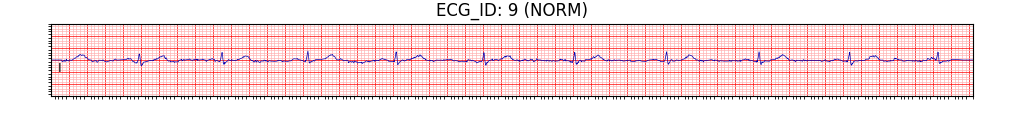
\includegraphics[width=0.95\textwidth]{Imagenes/Vectorial/Transformadas/NORM/ecg.png}
	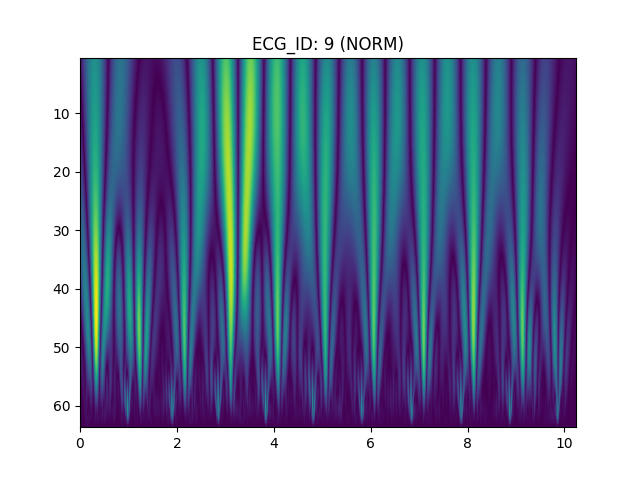
\includegraphics[width=0.45\textwidth]{Imagenes/Vectorial/Transformadas/NORM/cwt_ricker.png}
	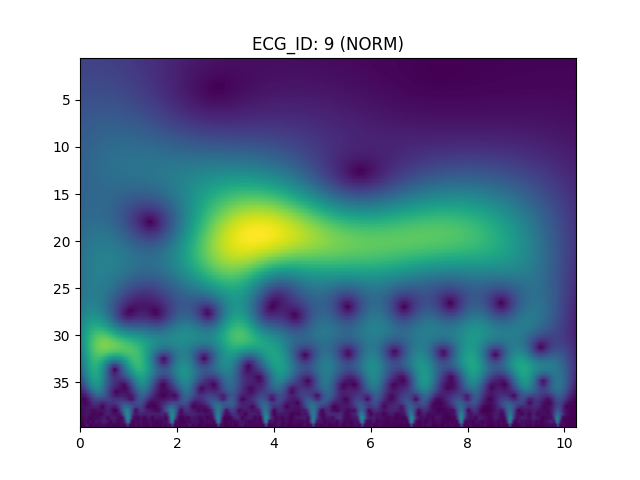
\includegraphics[width=0.45\textwidth]{Imagenes/Vectorial/Transformadas/NORM/cwt_morlet.png}
	\par Primera derivación de un ECG normal (arriba) y su transformada CWT con \emph{wavelet} de Ricker (izquierda) y Morlet (derecha).
	\caption{Transformadas CWT de la primera derivación de ECGs para cada clase.}
	\label{fig:cwt}
\end{figure}
\begin{figure}[t]\ContinuedFloat
	\centering
	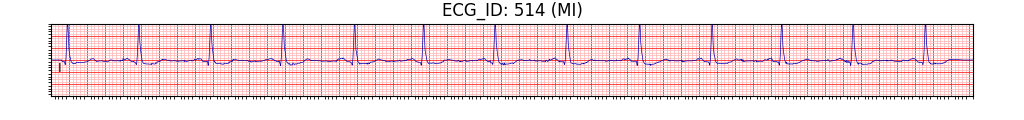
\includegraphics[width=0.95\textwidth]{Imagenes/Vectorial/Transformadas/MI/ecg.png}
	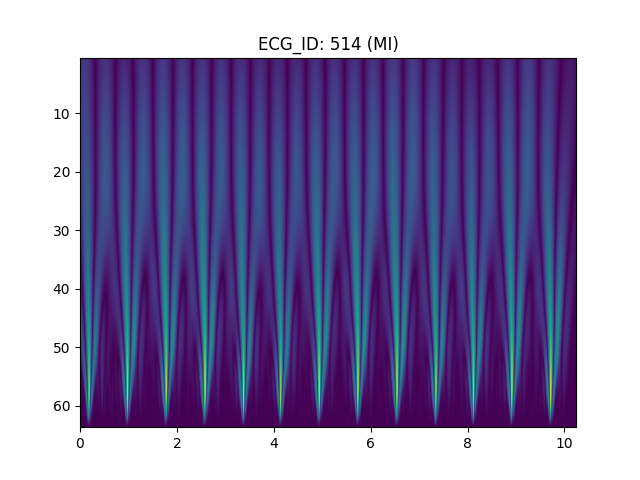
\includegraphics[width=0.45\textwidth]{Imagenes/Vectorial/Transformadas/MI/cwt_ricker.png}
	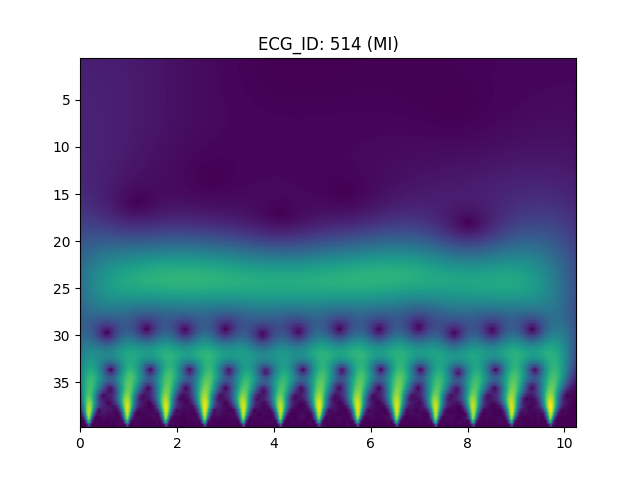
\includegraphics[width=0.45\textwidth]{Imagenes/Vectorial/Transformadas/MI/cwt_morlet.png}
	\par Primera derivación de un ECG de infarto de miocardio (arriba) y su transformada CWT con \emph{wavelet} de Ricker (izquierda) y Morlet (derecha).
	\vspace{1cm}

	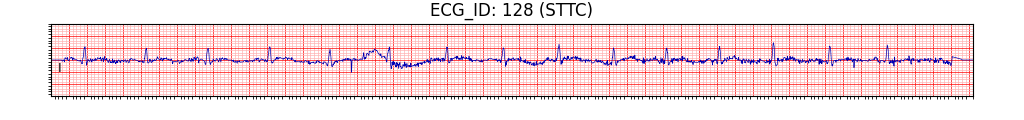
\includegraphics[width=0.95\textwidth]{Imagenes/Vectorial/Transformadas/STTC/ecg.png}
	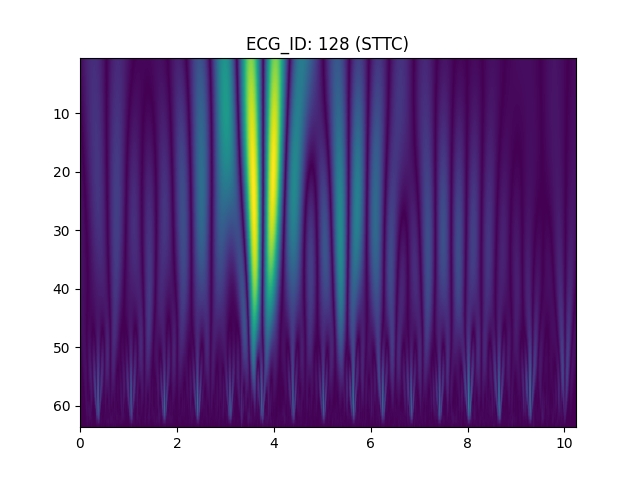
\includegraphics[width=0.45\textwidth]{Imagenes/Vectorial/Transformadas/STTC/cwt_ricker.png}
	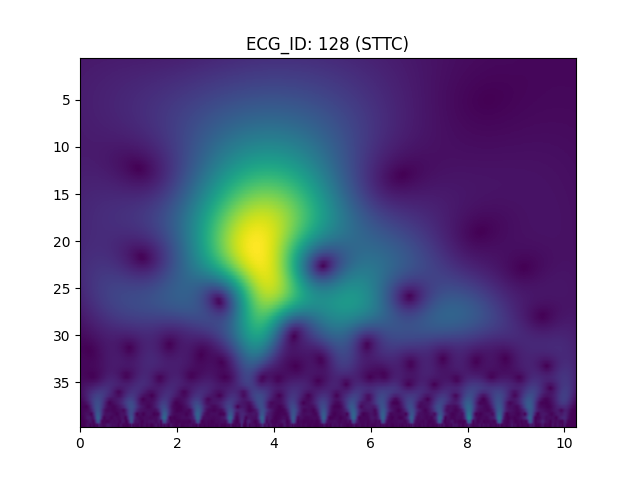
\includegraphics[width=0.45\textwidth]{Imagenes/Vectorial/Transformadas/STTC/cwt_morlet.png}
	\par Primera derivación de un ECG de tipo STTC (arriba) y su transformada CWT con \emph{wavelet} de Ricker (izquierda) y Morlet (derecha).
	\caption{Transformadas CWT de la primera derivación de ECGs para cada clase.}
\end{figure}
\begin{figure}[t]\ContinuedFloat
	\centering
	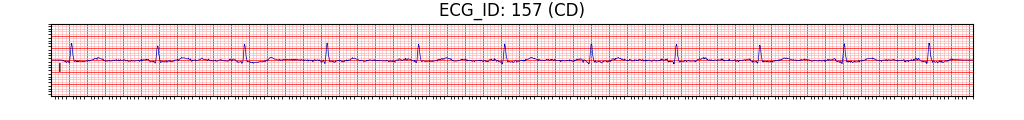
\includegraphics[width=0.95\textwidth]{Imagenes/Vectorial/Transformadas/CD/ecg.png}
	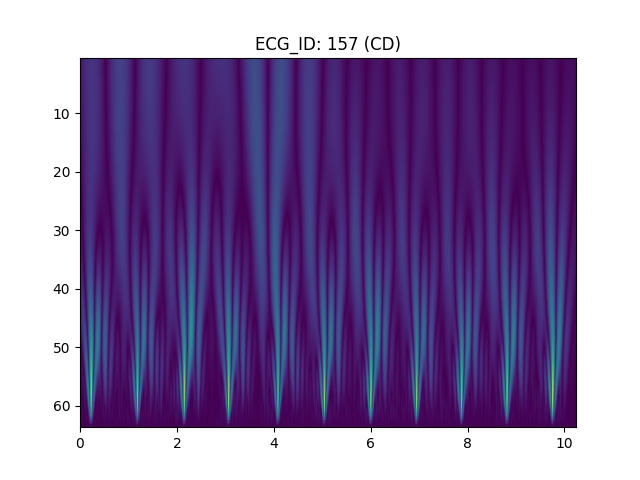
\includegraphics[width=0.45\textwidth]{Imagenes/Vectorial/Transformadas/CD/cwt_ricker.png}
	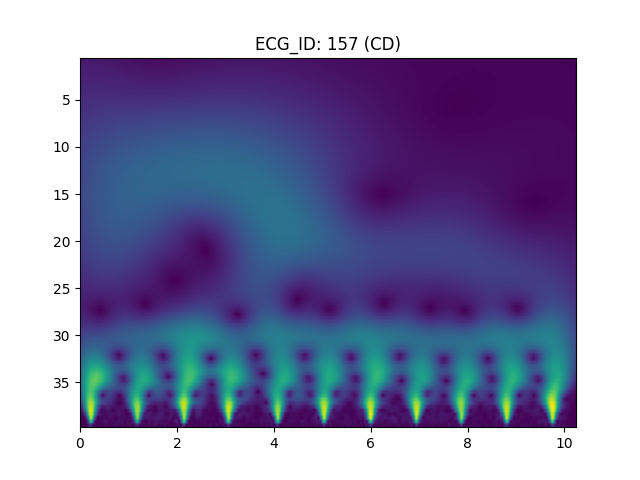
\includegraphics[width=0.45\textwidth]{Imagenes/Vectorial/Transformadas/CD/cwt_morlet.png}
	\par Primera derivación de un ECG de tipo CD (arriba) y su transformada CWT con \emph{wavelet} de Ricker (izquierda) y Morlet (derecha).
	\vspace{1cm}
	
	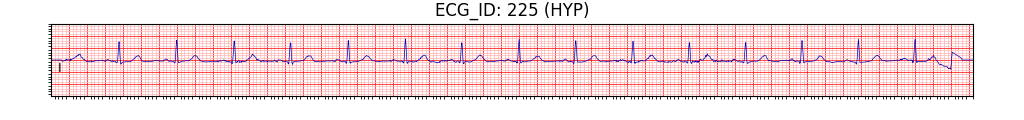
\includegraphics[width=0.95\textwidth]{Imagenes/Vectorial/Transformadas/HYP/ecg.png}
	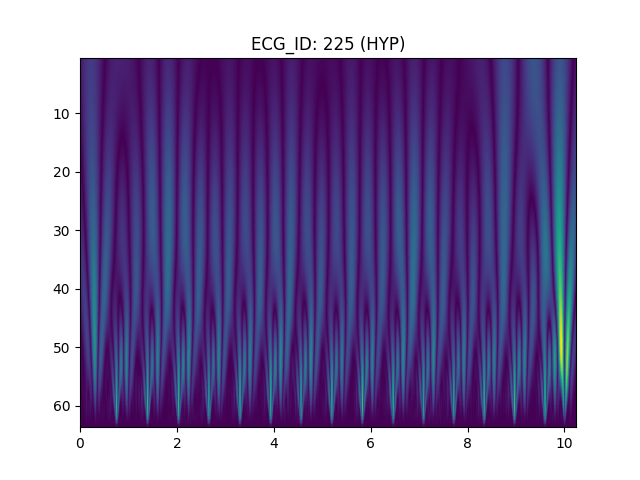
\includegraphics[width=0.45\textwidth]{Imagenes/Vectorial/Transformadas/HYP/cwt_ricker.png}
	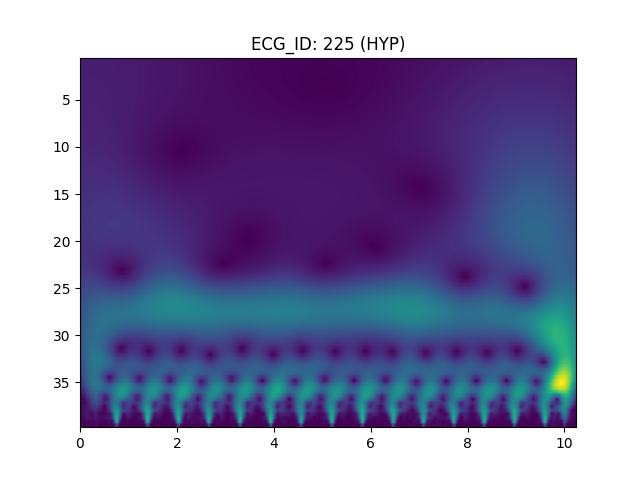
\includegraphics[width=0.45\textwidth]{Imagenes/Vectorial/Transformadas/HYP/cwt_morlet.png}
	\par Primera derivación de un ECG con hipertrofia (arriba) y su transformada CWT con \emph{wavelet} de Ricker (izquierda) y Morlet (derecha).
	\caption{Transformadas CWT de la primera derivación de ECGs para cada clase.}
\end{figure}
%\include{Capitulos/Capitulo4}
%\include{Capitulos/Capitulo5}
\chapter{Conclusiones y Trabajo Futuro}
\label{cap:conclusiones}

\section{Conclusiones}
A lo largo de este trabajo hemos demostrado que el modelo de Ribeiro funciona de manera adecuada aún entrenado con una base de datos más pequeña, lo que señala que es una arquitectura bastante sólida y prometedora.

No obstante, a la hora de introducir transformaciones, hemos descubierto que la arquitectura del modelo de Ribeiro no es adecuada para manejar imágenes, como es el caso de las transformadas. Esto no significa que el modelo de Ribeiro no pueda ser adaptado para trabajar con imágenes de manera adecuada, ya que una arquitectura con unos resultados tan buenos es muy prometedora.

Es importante señalar que el campo del \emph{deep learning} aplicado a la medicina es relativamente nuevo, y se publican trabajos innovadores y avances muy frecuentemente, por lo que el uso de transformadas para el análisis de ECGs sigue siendo una posible dirección de avance.

En cuanto a la explicabilidad, los \emph{saliency maps} basados en gradientes han mostrado ser un recurso prometedor para entender qué partes de la señal del ECG resultan relevantes para la red. Refinar estas explicaciones podría convertirlas en una herramienta de aprendizaje y educación útil tanto para estudiantes como para profesionales sanitarios que busquen familiarizarse con la IA. Además hemos visto como los profesionales reaccionaron muy positivamente a la existencia de herramientas que permitan explicar las decisiones de los modelos, y están convencidos de que, una vez se mejoren, van a ser un recurso muy importante en la educación.

\section{Trabajo futuro}
Dado el potencial del modelo y las limitaciones detectadas, se plantean varias líneas de trabajo para mejorar y ampliar los resultados:
\begin{enumerate}
	\item \textbf{Modificar la arquitectura para admitir capas Conv2D} \\
	Esta adaptación, si bien requeriría de un trabajo significativo, permitiría explotar mejor las ventajas de las transformaciones de la señal.
	\item \textbf{Explorar transformadas y parámetros adicionales} \\
	Siguiendo la línea anterior, una vez obtenida una arquitectura más adecuada para imágenes, podrían probarse otros parámetros a la hora de hacer las transformadas y estudiar su impacto.
	\item \textbf{Especializar el modelo en una anomalía} \\
	Transformar el modelo en un clasificador binario permitiría elegir los parámetros de las transformadas de manera más precisa, ya que distintas anomalías se manifiestan en distintas frecuencias.
	\item \textbf{Cambiar los umbrales de detección} \\
	En el trabajo de Ribeiro, en lugar de utilizar el umbral de 0.5 para clasificar las etiquetas, se calcularon los umbrales que optimizaban los resultados sobre el conjunto de validación. Esto es algo que, si bien en este trabajo no hemos abordado, podría mejorar los resultados de todos los modelos que hemos entrenado.
	\item \textbf{Delineación de señales en la explicación} \\
	Como señaló el experto, mediante delineación de señales podrían reducirse las explicaciones a dos latidos y asegurarse de que estas son homogéneas en ambos latidos. Estas mejoras harían viable el uso de estas explicaciones en el ámbito docente.
\end{enumerate}




\begin{otherlanguage}{english}
\chapter*{Introduction}
\label{cap:introduction}
\addcontentsline{toc}{chapter}{Introduction}
\section{Motivation}
AI has transformed numerous fields. In particular, the medical field has experienced significant advances through the application of artificial intelligence to diagnostics and data analysis. One of the most promising areas is the automated interpretation of signals in an ECG, which is essential for the early detection of heart diseases. Cardiovascular diseases are one of the leading causes of death globally \citep{whocvd}, highlighting the need for fast and accurate diagnostic methods.

The analysis of ECG's has historically been performed by healthcare professionals, such as cardiologists, due to the complexity and variability of the signals. However, this process is slow, costly, and highly dependent on the specialist’s experience. By adopting \emph{Deep Learning} models, such as convolutional neural networks (CNN), the goal is to automate and enhance this analysis, providing rapid results that, in many cases, are comparable to those obtained by human experts \citep{hannun_cardiologist_2019}. This approach not only promises to increase diagnostic efficiency but also improve accuracy and reduce the workload of medical staff.

Nevertheless, for these tools to gain trust in clinical settings and meet quality and ethical standards, they must be explainable \citep{Molnar2019}. The explainability of AI models permits understanding and justifying the decisions made during the analysis of cardiac signals, a critical factor in high-impact applications such as medicine, where an error can directly affect patient health \citep{Goodman2017}.

Throughout this work, we will explore various neural network architectures and signal transformation techniques to classify and detect abnormalities in ECGs, aiming to develop and refine an ECG classifier model for four groups of cardiac anomalies. In addition, we will incorporate explainability methods so that model results can be interpreted and validated by healthcare professionals, which is essential for clinical adoption of these technologies.

\section{Objectives}
The main objective of this work is to modify, train, and evaluate the model originally proposed by \cite{ribeiro} (hereinafter, the “original model”) by applying it to the public PTB-XL database \citep{ptbxldb}. To achieve this, we will introduce a modification in the model’s input layer that allows the inclusion of transforms (e.g., STFT or CWT) to investigate whether converting the signal into different representations can improve performance. However, no changes are made to the model’s internal architecture.

Based on the above, the specific objectives are:

\begin{enumerate}
	\item \textbf{Train the original model} using the PTB-XL database.
	\item \textbf{Modify the original model} so that it accepts signal transformations, permitting the training of alternative versions of the model with transformed data.
	\item \textbf{Compare the performance} of each variant with the original model using metrics such as F1-Score, analyzing whether the transformations are beneficial.
	\item \textbf{Apply an explainability method} so that a specialist can understand which parts of the ECG signal influence the prediction. For reasons to be discussed later, this will only be applied to the original model.
\end{enumerate}

\section{Document structure}
This document is organized into six chapters, whose contents are described below:
\begin{itemize}
	\item \textbf{Chapter 2: Estado del arte} \\
	Basic concepts related to electrocardiograms are presented, highlighting the importance of their waves (P, QRS, T) and the most common anomalies typically detected. Furthermore, the literature related to the use of neural networks in the analysis of ECG's is reviewed, and relevant databases (such as PTB-XL) are described.
	
	\item  \textbf{Chapter 3: Metodología y preparación de datos} \\
	The process for handling ECG's is detailed, including the division into training, validation, and test sets. In addition, the metrics used to evaluate the models and the transformations employed are described.
	
	\item \textbf{Chapter 4: Entrenamiento y resultados}\\
	The training conditions for each model (including modifications to the original model) and the libraries used are explained, and the quantitative results obtained through the metrics are presented and compared.
	
	\item \textbf{Chapter 5: Explicabilidad}\\
	The gradient-based \emph{saliency maps} explainability method applied to Ribeiro’s model is described. In addition, the perspective of a specialist physician analyzing the generated explanations is included, and reflections on the method and potential improvements are discussed.
	
	\item \textbf{Chapter 6: Conclusiones y trabajo futuro}\\
	The conclusions derived from the results are integrated, assessing the extent to which the stated objectives have been met. Furthermore, the main contributions of this work are identified, and future research directions are proposed (such as the inclusion of Conv2D layers).
\end{itemize}

Finally, a bibliography section is included, containing all the sources consulted throughout the document, as well as an appendix with the code used\footnote{All the content of this work can be found in \href{https://github.com/NotNoe/TFG-Info}{this GitHub repository}.} and another with the physician’s comments transcribed.



\chapter*{Conclusions and Future Work}
\label{cap:conclusions}
\addcontentsline{toc}{chapter}{Conclusions and Future Work}

Conclusions and future lines of work. This chapter contains the translation of Chapter \ref{cap:conclusiones}.



\end{otherlanguage}

%\chapter*{Contribuciones Personales}
\label{cap:contribucionesPersonales}
\addcontentsline{toc}{chapter}{Contribuciones Personales}

En caso de trabajos no unipersonales, cada participante indicará en la memoria su contribución al proyecto con una extensión de al menos dos páginas por cada uno de los participantes.

En caso de trabajo unipersonal, elimina esta página en el fichero \texttt{TFGTeXiS.tex} (comenta o borra la línea \verb|\chapter*{Contribuciones Personales}
\label{cap:contribucionesPersonales}
\addcontentsline{toc}{chapter}{Contribuciones Personales}

En caso de trabajos no unipersonales, cada participante indicará en la memoria su contribución al proyecto con una extensión de al menos dos páginas por cada uno de los participantes.

En caso de trabajo unipersonal, elimina esta página en el fichero \texttt{TFGTeXiS.tex} (comenta o borra la línea \verb|\chapter*{Contribuciones Personales}
\label{cap:contribucionesPersonales}
\addcontentsline{toc}{chapter}{Contribuciones Personales}

En caso de trabajos no unipersonales, cada participante indicará en la memoria su contribución al proyecto con una extensión de al menos dos páginas por cada uno de los participantes.

En caso de trabajo unipersonal, elimina esta página en el fichero \texttt{TFGTeXiS.tex} (comenta o borra la línea \verb|\include{Capitulos/ContribucionesPersonales}|).

\section*{Estudiante 1}
Al menos dos páginas con las contribuciones del estudiante 1.

\section*{Estudiante 2}
Al menos dos páginas con las contribuciones del estudiante 2. En caso de que haya más estudiantes, copia y pega una de estas secciones.

|).

\section*{Estudiante 1}
Al menos dos páginas con las contribuciones del estudiante 1.

\section*{Estudiante 2}
Al menos dos páginas con las contribuciones del estudiante 2. En caso de que haya más estudiantes, copia y pega una de estas secciones.

|).

\section*{Estudiante 1}
Al menos dos páginas con las contribuciones del estudiante 1.

\section*{Estudiante 2}
Al menos dos páginas con las contribuciones del estudiante 2. En caso de que haya más estudiantes, copia y pega una de estas secciones.



%
% Bibliografía
%
% Si el TFM se escribe en inglés, editar TeXiS/TeXiS_bib para cambiar el
% estilo de las referencias
%---------------------------------------------------------------------
%
%                      configBibliografia.tex
%
%---------------------------------------------------------------------
%
% bibliografia.tex
% Copyright 2009 Marco Antonio Gomez-Martin, Pedro Pablo Gomez-Martin
%
% This file belongs to the TeXiS manual, a LaTeX template for writting
% Thesis and other documents. The complete last TeXiS package can
% be obtained from http://gaia.fdi.ucm.es/projects/texis/
%
% Although the TeXiS template itself is distributed under the 
% conditions of the LaTeX Project Public License
% (http://www.latex-project.org/lppl.txt), the manual content
% uses the CC-BY-SA license that stays that you are free:
%
%    - to share & to copy, distribute and transmit the work
%    - to remix and to adapt the work
%
% under the following conditions:
%
%    - Attribution: you must attribute the work in the manner
%      specified by the author or licensor (but not in any way that
%      suggests that they endorse you or your use of the work).
%    - Share Alike: if you alter, transform, or build upon this
%      work, you may distribute the resulting work only under the
%      same, similar or a compatible license.
%
% The complete license is available in
% http://creativecommons.org/licenses/by-sa/3.0/legalcode
%
%---------------------------------------------------------------------
%
% Fichero  que  configura  los  parámetros  de  la  generación  de  la
% bibliografía.  Existen dos  parámetros configurables:  los ficheros
% .bib que se utilizan y la frase célebre que aparece justo antes de la
% primera referencia.
%
%---------------------------------------------------------------------


%%%%%%%%%%%%%%%%%%%%%%%%%%%%%%%%%%%%%%%%%%%%%%%%%%%%%%%%%%%%%%%%%%%%%%
% Definición de los ficheros .bib utilizados:
% \setBibFiles{<lista ficheros sin extension, separados por comas>}
% Nota:
% Es IMPORTANTE que los ficheros estén en la misma línea que
% el comando \setBibFiles. Si se desea utilizar varias líneas,
% terminarlas con una apertura de comentario.
%%%%%%%%%%%%%%%%%%%%%%%%%%%%%%%%%%%%%%%%%%%%%%%%%%%%%%%%%%%%%%%%%%%%%%
\setBibFiles{%
biblio%
}

%%%%%%%%%%%%%%%%%%%%%%%%%%%%%%%%%%%%%%%%%%%%%%%%%%%%%%%%%%%%%%%%%%%%%%
% Definición de la frase célebre para el capítulo de la
% bibliografía. Dentro normalmente se querrá hacer uso del entorno
% \begin{FraseCelebre}, que contendrá a su vez otros dos entornos,
% un \begin{Frase} y un \begin{Fuente}.
%
% Nota:
% Si no se quiere cita, se puede eliminar su definición (en la
% macro setCitaBibliografia{} ).
%%%%%%%%%%%%%%%%%%%%%%%%%%%%%%%%%%%%%%%%%%%%%%%%%%%%%%%%%%%%%%%%%%%%%%


%%
%% Creamos la bibliografia
%%
\makeBib

% Variable local para emacs, para  que encuentre el fichero maestro de
% compilación y funcionen mejor algunas teclas rápidas de AucTeX

%%%
%%% Local Variables:
%%% mode: latex
%%% TeX-master: "../Tesis.tex"
%%% End:



% Apéndices
\appendix
\chapter{Título del Apéndice A}
\label{Appendix:Key1}

Los apéndices son secciones al final del documento en las que se agrega texto con el objetivo de ampliar los contenidos del documento principal.
\chapter{Librerías utilizadas}
\label{anexo:librerias}

\begin{longtable}{|l|l|}
	\hline
	\textbf{Librería} & \textbf{Versión} \\ \hline
	\hline
	\endfirsthead
	\hline
	\textbf{Librería} & \textbf{Versión} \\ \hline
	\endhead
	\hline
	\endfoot
	\hline
	\endlastfoot
	\_libgcc\_mutex      & 0.1=main        \\ \hline
	\_openmp\_mutex      & 5.1=1\_gnu      \\ \hline
	bzip2                & 1.0.8=h7b6447c\_0 \\ \hline
	ca-certificates      & 2023.12.12=h06a4308\_0 \\ \hline
	ld\_impl\_linux-64   & 2.38=h1181459\_1 \\ \hline
	libffi               & 3.4.4=h6a678d5\_0 \\ \hline
	libgcc-ng            & 11.2.0=h1234567\_1 \\ \hline
	libgomp              & 11.2.0=h1234567\_1 \\ \hline
	libstdcxx-ng         & 11.2.0=h1234567\_1 \\ \hline
	libuuid              & 1.41.5=h5eee18b\_0 \\ \hline
	ncurses              & 6.4=h6a678d5\_0 \\ \hline
	openssl              & 3.0.13=h7f8727e\_0 \\ \hline
	pip                  & 23.3.1=py311h06a4308\_0 \\ \hline
	python               & 3.11.7=h955ad1f\_0 \\ \hline
	readline             & 8.2=h5eee18b\_0 \\ \hline
	setuptools           & 68.2.2=py311h06a4308\_0 \\ \hline
	sqlite               & 3.41.2=h5eee18b\_0 \\ \hline
	tk                   & 8.6.12=h1ccaba5\_0 \\ \hline
	wheel                & 0.41.2=py311h06a4308\_0 \\ \hline
	xz                   & 5.4.5=h5eee18b\_0 \\ \hline
	zlib                 & 1.2.13=h5eee18b\_0 \\ \hline
	absl-py              & 2.1.0 \\ \hline
	aiohttp              & 3.9.3 \\ \hline
	aiosignal            & 1.3.1 \\ \hline
	asttokens            & 2.4.1 \\ \hline
	astunparse           & 1.6.3 \\ \hline
	attrs                & 23.2.0 \\ \hline
	autograd             & 1.7.0 \\ \hline
	beautifulsoup4       & 4.12.3 \\ \hline
	bleach               & 6.1.0 \\ \hline
	cachetools           & 5.3.2 \\ \hline
	captum               & 0.7.0 \\ \hline
	certifi              & 2024.2.2 \\ \hline
	cffi                 & 1.16.0 \\ \hline
	charset-normalizer   & 3.3.2 \\ \hline
	cloudpickle          & 3.1.0 \\ \hline
	comm                 & 0.2.1 \\ \hline
	contourpy            & 1.2.0 \\ \hline
	cycler               & 0.12.1 \\ \hline
	deap                 & 1.4.1 \\ \hline
	debugpy              & 1.8.0 \\ \hline
	decorator            & 5.1.1 \\ \hline
	defusedxml           & 0.7.1 \\ \hline
	deprecated           & 1.2.13 \\ \hline
	ecg-plot             & 0.2.8 \\ \hline
	et-xmlfile           & 1.1.0 \\ \hline
	executing            & 2.0.1 \\ \hline
	fastjsonschema       & 2.19.1 \\ \hline
	filelock             & 3.13.4 \\ \hline
	flatbuffers          & 23.5.26 \\ \hline
	fonttools            & 4.48.1 \\ \hline
	frozenlist           & 1.4.1 \\ \hline
	fsspec               & 2024.3.1 \\ \hline
	gast                 & 0.5.4 \\ \hline
	google-auth          & 2.27.0 \\ \hline
	google-auth-oauthlib & 1.2.0 \\ \hline
	google-pasta         & 0.2.0 \\ \hline
	grpcio               & 1.60.1 \\ \hline
	h5py                 & 3.10.0 \\ \hline
	idna                 & 3.6 \\ \hline
	ipykernel            & 6.29.2 \\ \hline
	ipython              & 8.21.0 \\ \hline
	jedi                 & 0.19.1 \\ \hline
	jinja2               & 3.1.3 \\ \hline
	joblib               & 1.3.2 \\ \hline
	jsonschema           & 4.21.1 \\ \hline
	jsonschema-specifications & 2023.12.1 \\ \hline
	jupyter-client       & 8.6.0 \\ \hline
	jupyter-core         & 5.7.1 \\ \hline
	jupyterlab-pygments  & 0.3.0 \\ \hline
	keras                & 2.15.0 \\ \hline
	kiwisolver           & 1.4.5 \\ \hline
	libclang             & 16.0.6 \\ \hline
	lightning-utilities  & 0.11.2 \\ \hline
	llvmlite             & 0.43.0 \\ \hline
	locket               & 1.0.0 \\ \hline
	markdown             & 3.3.4 \\ \hline
	markupsafe           & 2.1.5 \\ \hline
	matplotlib           & 3.8.2 \\ \hline
	matplotlib-inline    & 0.1.6 \\ \hline
	mistune              & 3.0.2 \\ \hline
	ml-dtypes            & 0.2.0 \\ \hline
	mpmath               & 1.3.0 \\ \hline
	multidict            & 6.0.5 \\ \hline
	nbclient             & 0.9.0 \\ \hline
	nbconvert            & 7.16.1 \\ \hline
	nbformat             & 5.9.2 \\ \hline
	nest-asyncio         & 1.6.0 \\ \hline
	networkx             & 3.3 \\ \hline
	numba                & 0.60.0 \\ \hline
	numpy                & 1.26.4 \\ \hline
	nvidia-cublas-cu12   & 12.1.3.1 \\ \hline
	nvidia-cuda-cupti-cu12 & 12.1.105 \\ \hline
	nvidia-cuda-nvcc-cu12 & 12.2.140 \\ \hline
	nvidia-cuda-nvrtc-cu12 & 12.1.105 \\ \hline
	nvidia-cuda-runtime-cu12 & 12.1.105 \\ \hline
	nvidia-cudnn-cu12    & 8.9.2.26 \\ \hline
	nvidia-cufft-cu12    & 11.0.2.54 \\ \hline
	nvidia-curand-cu12   & 10.3.2.106 \\ \hline
	nvidia-cusolver-cu12 & 11.4.5.107 \\ \hline
	nvidia-cusparse-cu12 & 12.1.0.106 \\ \hline
	nvidia-nccl-cu12     & 2.19.3 \\ \hline
	nvidia-nvjitlink-cu12 & 12.2.140 \\ \hline
	nvidia-nvtx-cu12     & 12.1.105 \\ \hline
	oauthlib             & 3.2.2 \\ \hline
	opencv-python        & 4.6.0.66 \\ \hline
	openpyxl             & 3.1.2 \\ \hline
	opt-einsum           & 3.3.0 \\ \hline
	packaging            & 23.2 \\ \hline
	pandas               & 2.2.0 \\ \hline
	pandocfilters        & 1.5.1 \\ \hline
	parso                & 0.8.3 \\ \hline
	partd                & 1.2.0 \\ \hline
	patsy                & 1.0.1 \\ \hline
	pexpect              & 4.9.0 \\ \hline
	pillow               & 10.2.0 \\ \hline
	platformdirs         & 4.2.0 \\ \hline
	prompt-toolkit       & 3.0.43 \\ \hline
	protobuf             & 4.23.4 \\ \hline
	psutil               & 5.9.8 \\ \hline
	ptyprocess           & 0.7.0 \\ \hline
	pure-eval            & 0.2.2 \\ \hline
	pyaml                & 24.9.0 \\ \hline
	pyarrow              & 15.0.2 \\ \hline
	pyasn1               & 0.5.1 \\ \hline
	pyasn1-modules       & 0.3.0 \\ \hline
	pycparser            & 2.21 \\ \hline
	pygments             & 2.17.2 \\ \hline
	pymop                & 0.2.4 \\ \hline
	pyparsing            & 3.1.1 \\ \hline
	python-dateutil      & 2.8.2 \\ \hline
	pytorch-lightning    & 2.2.1 \\ \hline
	pyts                 & 0.13.0 \\ \hline
	pytz                 & 2024.1 \\ \hline
	pyyaml               & 6.0.1 \\ \hline
	pyzmq                & 25.1.2 \\ \hline
	referencing          & 0.33.0 \\ \hline
	requests             & 2.31.0 \\ \hline
	requests-oauthlib    & 1.3.1 \\ \hline
	rpds-py              & 0.18.0 \\ \hline
	rsa                  & 4.9 \\ \hline
	scikit-base          & 0.11.0 \\ \hline
	scikit-learn         & 1.3.0 \\ \hline
	scikit-optimize      & 0.10.2 \\ \hline
	scipy                & 1.14.1 \\ \hline
	seaborn              & 0.13.2 \\ \hline
	shap                 & 0.46.0 \\ \hline
	six                  & 1.16.0 \\ \hline
	sktime               & 0.34.1 \\ \hline
	slicer               & 0.0.8 \\ \hline
	soundfile            & 0.12.1 \\ \hline
	soupsieve            & 2.5 \\ \hline
	stack-data           & 0.6.3 \\ \hline
	statsmodels          & 0.14.4 \\ \hline
	stumpy               & 1.13.0 \\ \hline
	sympy                & 1.12 \\ \hline
	tensorboard          & 2.15.1 \\ \hline
	tensorboard-data-server & 0.7.2 \\ \hline
	tensorflow           & 2.15.0.post1 \\ \hline
	tensorflow-estimator & 2.15.0 \\ \hline
	tensorflow-io-gcs-filesystem & 0.36.0 \\ \hline
	termcolor            & 2.4.0 \\ \hline
	tf-explain           & 0.3.1 \\ \hline
	threadpoolctl        & 3.2.0 \\ \hline
	tinycss2             & 1.2.1 \\ \hline
	toolz                & 1.0.0 \\ \hline
	torch                & 2.2.2 \\ \hline
	torchcam             & 0.4.0 \\ \hline
	torchmetrics         & 1.3.2 \\ \hline
	tornado              & 6.4 \\ \hline
	tqdm                 & 4.65.2 \\ \hline
	traitlets            & 5.14.1 \\ \hline
	triton               & 2.2.0 \\ \hline
	tsfresh              & 0.20.3 \\ \hline
	tsinterpret          & 0.4.7 \\ \hline
	tslearn              & 0.6.3 \\ \hline
	typing-extensions    & 4.9.0 \\ \hline
	tzdata               & 2023.4 \\ \hline
	urllib3              & 2.2.0 \\ \hline
	wcwidth              & 0.2.13 \\ \hline
	webencodings         & 0.5.1 \\ \hline
	werkzeug             & 3.0.1 \\ \hline
	wfdb                 & 4.1.2 \\ \hline
	wrapt                & 1.14.1 \\ \hline
	xarray               & 2024.3.0 \\ \hline
	xmljson              & 0.2.1 \\ \hline
	yarl                 & 1.9.4 \\ \hline
\end{longtable}
%\include{Apendices/appendixC}
%\include{...}
%\include{...}
%\include{...}
\backmatter



%
% Índice de palabras
%

% Sólo  la   generamos  si  está   declarada  \generaindice.  Consulta
% TeXiS.sty para más información.

% En realidad, el soporte para la generación de índices de palabras
% en TeXiS no está documentada en el manual, porque no ha sido usada
% "en producción". Por tanto, el fichero que genera el índice
% *no* se incluye aquí (está comentado). Consulta la documentación
% en TeXiS_pream.tex para más información.
\ifx\generaindice\undefined
\else
%%---------------------------------------------------------------------
%
%                        TeXiS_indice.tex
%
%---------------------------------------------------------------------
%
% TeXiS_indice.tex
% Copyright 2009 Marco Antonio Gomez-Martin, Pedro Pablo Gomez-Martin
%
% This file belongs to TeXiS, a LaTeX template for writting
% Thesis and other documents. The complete last TeXiS package can
% be obtained from http://gaia.fdi.ucm.es/projects/texis/
%
% This work may be distributed and/or modified under the
% conditions of the LaTeX Project Public License, either version 1.3
% of this license or (at your option) any later version.
% The latest version of this license is in
%   http://www.latex-project.org/lppl.txt
% and version 1.3 or later is part of all distributions of LaTeX
% version 2005/12/01 or later.
%
% This work has the LPPL maintenance status `maintained'.
% 
% The Current Maintainers of this work are Marco Antonio Gomez-Martin
% and Pedro Pablo Gomez-Martin
%
%---------------------------------------------------------------------
%
% Contiene  los  comandos  para  generar  el índice  de  palabras  del
% documento.
%
%---------------------------------------------------------------------
%
% NOTA IMPORTANTE: el  soporte en TeXiS para el  índice de palabras es
% embrionario, y  de hecho  ni siquiera se  describe en el  manual. Se
% proporciona  una infraestructura  básica (sin  terminar)  para ello,
% pero  no ha  sido usada  "en producción".  De hecho,  a pesar  de la
% existencia de  este fichero, *no* se incluye  en Tesis.tex. Consulta
% la documentación en TeXiS_pream.tex para más información.
%
%---------------------------------------------------------------------


% Si se  va a generar  la tabla de  contenidos (el índice  habitual) y
% también vamos a  generar el índice de palabras  (ambas decisiones se
% toman en  función de  la definición  o no de  un par  de constantes,
% puedes consultar modo.tex para más información), entonces metemos en
% la tabla de contenidos una  entrada para marcar la página donde está
% el índice de palabras.

\ifx\generatoc\undefined
\else
   \addcontentsline{toc}{chapter}{\indexname}
\fi


% Generamos el índice
\printindex

% Variable local para emacs, para  que encuentre el fichero maestro de
% compilación y funcionen mejor algunas teclas rápidas de AucTeX

%%%
%%% Local Variables:
%%% mode: latex
%%% TeX-master: "./tesis.tex"
%%% End:

\fi

%
% Lista de acrónimos
%

% Sólo  lo  generamos  si  está declarada  \generaacronimos.  Consulta
% TeXiS.sty para más información.


\ifx\generaacronimos\undefined
\else
%---------------------------------------------------------------------
%
%                        TeXiS_acron.tex
%
%---------------------------------------------------------------------
%
% TeXiS_acron.tex
% Copyright 2009 Marco Antonio Gomez-Martin, Pedro Pablo Gomez-Martin
%
% This file belongs to TeXiS, a LaTeX template for writting
% Thesis and other documents. The complete last TeXiS package can
% be obtained from http://gaia.fdi.ucm.es/projects/texis/
%
% This work may be distributed and/or modified under the
% conditions of the LaTeX Project Public License, either version 1.3
% of this license or (at your option) any later version.
% The latest version of this license is in
%   http://www.latex-project.org/lppl.txt
% and version 1.3 or later is part of all distributions of LaTeX
% version 2005/12/01 or later.
%
% This work has the LPPL maintenance status `maintained'.
% 
% The Current Maintainers of this work are Marco Antonio Gomez-Martin
% and Pedro Pablo Gomez-Martin
%
%---------------------------------------------------------------------
%
% Contiene  los  comandos  para  generar  el listado de acrónimos
% documento.
%
%---------------------------------------------------------------------
%
% NOTA IMPORTANTE:  para que la  generación de acrónimos  funcione, al
% menos  debe  existir  un  acrónimo   en  el  documento.  Si  no,  la
% compilación  del   fichero  LaTeX  falla  con   un  error  "extraño"
% (indicando  que  quizá  falte  un \item).   Consulta  el  comentario
% referente al paquete glosstex en TeXiS_pream.tex.
%
%---------------------------------------------------------------------


% Redefinimos a español  el título de la lista  de acrónimos (Babel no
% lo hace por nosotros esta vez)

\def\listacronymname{Lista de acrónimos}

% Para el glosario:
% \def\glosarryname{Glosario}

% Si se  va a generar  la tabla de  contenidos (el índice  habitual) y
% también vamos a  generar la lista de acrónimos  (ambas decisiones se
% toman en  función de  la definición  o no de  un par  de constantes,
% puedes consultar config.tex  para más información), entonces metemos
% en la  tabla de contenidos una  entrada para marcar  la página donde
% está el índice de palabras.

\ifx\generatoc\undefined
\else
   \addcontentsline{toc}{chapter}{\listacronymname}
\fi


% Generamos la lista de acrónimos (en realidad el índice asociado a la
% lista "acr" de GlossTeX)

\printglosstex(acr)

% Variable local para emacs, para  que encuentre el fichero maestro de
% compilación y funcionen mejor algunas teclas rápidas de AucTeX

%%%
%%% Local Variables:
%%% mode: latex
%%% TeX-master: "../Tesis.tex"
%%% End:

\fi

%
% Final
%
%---------------------------------------------------------------------
%
%                      fin.tex
%
%---------------------------------------------------------------------
%
% fin.tex
% Copyright 2009 Marco Antonio Gomez-Martin, Pedro Pablo Gomez-Martin
%
% This file belongs to the TeXiS manual, a LaTeX template for writting
% Thesis and other documents. The complete last TeXiS package can
% be obtained from http://gaia.fdi.ucm.es/projects/texis/
%
% Although the TeXiS template itself is distributed under the 
% conditions of the LaTeX Project Public License
% (http://www.latex-project.org/lppl.txt), the manual content
% uses the CC-BY-SA license that stays that you are free:
%
%    - to share & to copy, distribute and transmit the work
%    - to remix and to adapt the work
%
% under the following conditions:
%
%    - Attribution: you must attribute the work in the manner
%      specified by the author or licensor (but not in any way that
%      suggests that they endorse you or your use of the work).
%    - Share Alike: if you alter, transform, or build upon this
%      work, you may distribute the resulting work only under the
%      same, similar or a compatible license.
%
% The complete license is available in
% http://creativecommons.org/licenses/by-sa/3.0/legalcode
%
%---------------------------------------------------------------------
%
% Contiene la última página
%
%---------------------------------------------------------------------


% Ponemos el marcador en el PDF
\ifpdf
   \pdfbookmark{Fin}{fin}
\fi

\thispagestyle{empty}\mbox{}

Este texto se puede encontrar en el fichero Cascaras/fin.tex. Si deseas eliminarlo, basta con comentar la línea correspondiente al final del fichero TFGTeXiS.tex.

\vspace*{4cm}

\small

\hfill \emph{--¿Qué te parece desto, Sancho? -- Dijo Don Quijote --}

\hfill \emph{Bien podrán los encantadores quitarme la ventura,}

\hfill \emph{pero el esfuerzo y el ánimo, será imposible.}

\hfill 

\hfill \emph{Segunda parte del Ingenioso Caballero} 

\hfill \emph{Don Quijote de la Mancha}

\hfill \emph{Miguel de Cervantes}

\vfill%space*{4cm}

\hfill \emph{--Buena está -- dijo Sancho --; fírmela vuestra merced.}

\hfill \emph{--No es menester firmarla -- dijo Don Quijote--,}

\hfill \emph{sino solamente poner mi rúbrica.}

\hfill 

\hfill \emph{Primera parte del Ingenioso Caballero} 

\hfill \emph{Don Quijote de la Mancha}

\hfill \emph{Miguel de Cervantes}


\newpage
\thispagestyle{empty}\mbox{}

\newpage

% Variable local para emacs, para  que encuentre el fichero maestro de
% compilación y funcionen mejor algunas teclas rápidas de AucTeX

%%%
%%% Local Variables:
%%% mode: latex
%%% TeX-master: "../Tesis.tex"
%%% End:

\end{document}
